% @Author: john
% @Date:   2016-02-27 08:36:03
% @Last Modified by:   John Hammond
% @Last Modified time: 2016-12-13 02:51:59

\documentclass[11pt]{article}
\usepackage{graphicx}

\topmargin -3cm

\usepackage[pdftex, pdfborderstyle={/S/U/W 0}]{hyperref} % this disables the boxes around links
\usepackage{amsmath}
\usepackage{xcolor}
\usepackage{fancyhdr}


\rhead{John Hammond 2016}

\definecolor{codegreen}{rgb}{0,0.6,0}
\definecolor{codegray}{rgb}{0.5,0.5,0.5}
\definecolor{codepurple}{rgb}{0.58,0,0.82}
\definecolor{backcolour}{rgb}{0.95,0.95,0.95}

\usepackage{listings}
\lstset{basicstyle=\ttfamily,
	showstringspaces=false,
	backgroundcolor=\color{backcolour},   
    commentstyle=\color{codegreen},
    keywordstyle=\color{magenta},
    numberstyle=\tiny\color{codegray},
    stringstyle=\color{codepurple},
    % basicstyle=\footnotesize,
	breaklines=true,                 
	captionpos=b,                    
	keepspaces=true,                 
	numbers=left,                    
	numbersep=5pt,                  
	showspaces=false,                
	showstringspaces=false,
	showtabs=false,                  
	tabsize=2
}
\usepackage[letterpaper, portrait, margin=1.15in, top=.75in]{geometry}
\usepackage[english]{babel}
\usepackage[utf8]{inputenc}
\pagestyle{fancy}

% \usepackage{hyperref}
% \hypersetup{colorlinks=true,pdfborderstyle={/S/U}}
\AtBeginDocument{\let\textlabel\label}

\title{  {\bf UNITED STATES COAST GUARD ACADEMY } }
\author{ { \bf INTRODUCTION TO LINUX } \\ { \bf COURSE AND MATERIALS } }
\date{}

\begin{document}
	
	\pagenumbering{gobble}
	\maketitle

	\begin{center}
		\graphicspath{ {.} }
		
\includegraphics[width=\textwidth,height=\textheight,keepaspectratio]{logo.png}
		\centering
		\vfill
		December 2016 \\
		John Hammond
	\end{center}

	\newpage

	% \hrulefill
	\renewcommand*\contentsname{Table of Contents}
	\tableofcontents
	\vfill
	\hrulefill

	\newpage

	\pagenumbering{arabic}

	\section{Introduction}
	\label{Introduction}
	\paragraph{} This document is my attempt to compile and archive all of the material and content that I developed for the 2016 ``Intro to Linux'' course that was offered within the Electrical Engineering department here at the United States Coast Guard Academy. The class was a one-credit course offered during the fall semester, that met in McAllister Hall room 208, co-taught by myself and LCDR Grant Wyman.

	\paragraph{} The resource is meant to be supplemented by an online archive and repository, available at \href{https://github.com/macee/linux_16}{https://github.com/macee/linux\_16}. The repository has been in flux and may not be as ``clean and orderly'' as this formal document hopes to be.

	\subsection{Author's Note}
	\label{Authors_Note}
	
	\paragraph{} The plan for the Intro to Linux course for the 2016 Fall Semester was that myself and LCDR Wyman would ``co-teach'' the class. What that really means is that LCDR Wyman would help with admin work, while I carved out a curriculum and developed learning software and exercises as a vessel for teaching very hands-on and technical content.

	\paragraph{} In place was a contract where I would develop the course and flesh it out into an extensible and reusable product; I would compile a formal guide and documentation for how to use the content I created for later years, and of course, tweak, tailor, and change things as the instructor sees fit.

	\paragraph{} In the ``Capture the Flag'' scene, which is a large culture for cyber security specialists and hackers, this is synonymous to what they call a \textit{writeup}. After solving some kind of technical challenge or problem, they explain their thought-process when looking at the problem, they share their code and any material they created to solve the problem, and then they show and explain how their solution works. 

	\paragraph{} This is my formal writeup.

	\paragraph{} I hope you enjoy.

	\begin{center}
		\graphicspath{ {.} }
		
\includegraphics[width=300px,height=200px,keepaspectratio]{tux.jpg}
		\centering
		\vfill
	\end{center}


	\section{The Raspberry Pi}

	\paragraph{} The Intro to Linux class made use of the small and inexpensive microcomputer, the Raspberry Pi.

	\paragraph{} Initially, this was to wow the students with the feasibility that such a computer could be so small, how it could run a full desktop-environment with Linux, and other neat bromides to try and interest a student who has been familiar with only the Windows operating system their whole life.

	\paragraph{} Reflecting on the course, the use of the Raspberry Pi was both good and bad.

	\begin{center}
		\graphicspath{ {.} }
		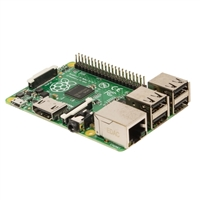
\includegraphics[width=300px,height=200px,keepaspectratio]{pi.jpg}
		\centering
	\end{center}

	\subsection{Advantages}

	The Raspberry Pi was a nicety in the following ways:

	\begin{itemize}
		\item Because the EE section has so many Raspberry Pi's, it was easy to get everyone up and running with a Linux distro very quickly.
		
		\item It created some more hands-on activity each day, letting the student put together their computer whenever they wanted to work (this doubles as negative)
	\end{itemize}

	\subsection{Disadvantages}

	Despite the benefits of using the small device, it was very easy to run into a few hiccups.

	\begin{itemize}
		\item Many students had trouble getting their VGA monitor to actually \textit{display}. This was a weekly occurrence. It typically took an instructor to intervene and try and remedy the problem themselves. 

		\item One student had struggled with the set up of the Raspberry Pi's so frequently that he went through four different devices in a day; myself and LCDR Wyman couldn't troubleshoot the first couple enough to get a display.
		
		\item Some operations on the Raspberry Pi are much slower considering its CPU power. Things like compiling software packages or installing software typically take a few minutes on the small chip, when on a typical Linux box they take only seconds.
		
		\item The Raspberry Pi initially has a different keyboard layout than what is used in the United States. Sure, we could cook solutions to this, but honestly you would be trying to solve a problem that doesn't have to be there in the first place.
	\end{itemize}

	\subsection{Future Recommendations}

	\paragraph{} I will take some author liberties here and actually recommend that for a future class that teaches Linux, make the use of the Raspberry Pi only a temporary thing. In my opinion, for actual \textit{use} of the Linux operating system, it is more important to have a stable machine that students can quickly boot up and is much faster with more modern repository packages. 

	\paragraph{} From a content-creator's perspective, the Raspberry Pi was a bit of a stumbling block. Myself being a Linux user, I run an Ubuntu Desktop on a typical Intel processor. Needless to say, this is the typical ``modern'' and ``mainstream'' Linux distribution that most old-Windows users convert to when they start to use Linux. Regardless, since I develop content in that environment, I would have to ``cross-check'' or verify success on the Raspbery Pi.  


	\begin{center}
		\graphicspath{ {.} }
		
\includegraphics[width=200px,height=200px,keepaspectratio]{ubuntu_logo.png}
		\centering
	\end{center}

	\paragraph{} There were a few occasions where I had compiled some binaries and forgot that the architecture was different on the Raspberry Pi, or didn't realize that some software package repositories weren't available on the Pi.

	\paragraph{} I cannot deny that the novelty of the Raspberry Pi is an attractive thing. In that regard I would recommend using it for maybe the first week or two of a future Linux class, but perhaps then moving on to a more common end-user distribution for the students to learn on. 

	\subsection{Hardware \& Equipment}

	\paragraph{} So for the actual use of the Raspberry Pi, we needed a...

	\begin{itemize}
		\item MicroUSB / AC adapter
		\item Ethernet Cable
		\item HDMI-to-VGA adapter
		\item MicroSD Card
		\item USB Mouse \& Keyboard
	\end{itemize}

	\subsection{Wireless Optional}

	\paragraph{} For the Raspberry Pi's, we used an Ethernet cable for wired Internet connection. You \textit{could} setup a wireless connection if you wanted to. I believe some of the newer models of the Raspberry Pi support wireless by default, but the models that we used for class we need a USB adapter, which would also have to be configured.

	\paragraph{} For scalability, I am unaware if it is feasible to automate the setup and configuration of the wireless USB adapter before installing the Raspbian image on the SD card... but afterwards, you could create a script to do what you need and push it out to the class by the github repo or any other means. You would have to trust the user-interaction and ask them to run the script, but you as the instructor can do obviously whatever you want. 

	\subsection{HDMI Output}

	\paragraph{} The monitors in the McAllister Hall Room 208 space that we used for this past semester only have DVI and VGA inputs. The Raspberry Pi models we were using only have an HDMI output. Because of this, we used an HDMI-to-VGA converter for every single device. This wasn't \textit{too much} of an issue; but it did add another step of troubleshooting when we couldn't get a display up on some students' device (which \textit{was} an issue).

	\paragraph{} If you care to remedy this you obviously have some options,  whether it be using a different room or different monitors or different devices entirely.

	\section{The Github Repository}

	\paragraph{} The Electrical Engineering department within the US Coast Guard Academy owns an academic license for \href{http://github.com}{http://github.com}, which allows the organization to create however many private and public repositories they would like.

	\paragraph{} This is taken advantage of in many other classes, but most others tend to really stumble when trying to push or pull content to and from github. The best way to manage digital content with github is through the command-line interface where command-line use was already an integral part of the Intro to Linux course. 

	\subsection{Students' Private Repositories}

	\paragraph{} Under the "MacEE" Github license, each student was able to their own private repository, typically titled with their last name (as an example, mine is \href{https://github.com/macee/Hammond}{https://github.com/macee/Hammond}). It was expected that students would have their own personal repository cloned and accessible in their Linux home directory. This was used to write reflections or post any code or files that was asked of the students during class. 

	\subsection{Class Public Repository}

	\paragraph{} For the 2016 Intro to Linux course, we created a specific \texttt{linux\_16} Github repository. This was made public and it housed all the code, content, and material for the course. As the content creator, this was what allowed me to easily push things to students computers. 

	\paragraph{} To adopt the Linux open-source mindset, it was my goal to ensure that repository was left public and included all of the source code and ``setup'' or ``build'' material, for everything we had done in class. I occasionally would remind students that all that content is there for their viewing pleasure, in case they were more curious how some of the training tools or the exercises worked --- but I am doubtful any students really dove deeper into it. On principle, anyway, I wanted it all to be available.


	\section{Raspbian Setup Script}

	\paragraph{} We had just over a dozen students in the 2016 Intro to Linux class. This was great; but it also meant we had to prep more than a dozen Raspberry Pi's. You could consider this another reason why I recommend against using the Pi permanently for future classes --- but I digress.

	\paragraph{} So when we were prepping the course, the initial goal was to have each Raspberry Pi be installed with a fresh image of Raspbian. 


	\subsection{The MicroSD cards} 

	\paragraph{} The Raspberry Pi uses a MicroSD card as its ``hard-drive'' by default; so we had to cook Raspbian on over twelve different cards.

	\paragraph{} To work with the MicroSD cards, I needed an adapter to be able to work with the drive on my own laptop; my machine only has a regular-size SD card reader. This wasn't an issue; we had plenty of adapters; but keep in mind that is another piece of equipment you will need if you ever do these same tasks.

	\subsection{Background Information}

	\paragraph{} Needless to say, installing Raspbian on all of the MicroSD cards ``by hand'' would be very tedious. So, just to speed things along, I wrote just a small and simple script to automate the process. Now, all it took was placing the SD Card into my machine, running the script, waiting a few minutes and we were done! A new Raspbian drive was cooked and ready to go. We could swap in a new card, run the script again ... and repeat as necessary.

	\paragraph{} Again, the script is simple; it really just automates the commands given in the online documentation for setting up Raspbian: \href{https://www.raspberrypi.org/documentation/installation/installing-images/linux.md}{https://www.raspberrypi.org/documentation/installation/installing-images/linux.md}

	\paragraph{} For completeness, the whole script is attached here, on its own dedicated page.

	\newpage

	\subsection{Raspbian Setup Source Code}

	\begin{lstlisting}[language=Bash]
#!/bin/bash

RASPBIAN_FILENAME="raspbian_latest.img"
MICROSD_DEVICE="/dev/mmcblk0"

# Check to see any microSD cards. If you see any, umount them
df -h |grep "$MICROSD_DEVICE"|cut -d " " -f1|while read line; do umount $line; done

# Do we have the IMG file?
if [ -e "$RASPBIAN_FILENAME" ]
then
	# If we do, start to burn it to the MicroSD card.
	dd bs=4M if="$RASPBIAN_FILENAME" of="$MICROSD_DEVICE"
else
	# If not, do we have the zip file?
	if [ -e "${RASPBIAN_FILENAME/.img/.zip}" ]
	then
		# If we do, unzip the zip file.
		unzip -P "${RASPBIAN_FILENAME/.img/.zip}" > "${RASPBIAN_FILENAME}"
		# If we do, start to burn it to the MicroSD card.
		dd bs=4M if="$RASPBIAN_FILENAME" of="$MICROSD_DEVICE"
	else
		# If not, download the zip file.
		wget "https://downloads.raspberrypi.org/raspbian_latest" -O "${RASPBIAN_FILENAME/.img/.zip}"
		# unzip it.
		unzip -P "${RASPBIAN_FILENAME/.img/.zip}" > "${RASPBIAN_FILENAME}"
		# flash the drive
		dd bs=4M if="$RASPBIAN_FILENAME" of="$MICROSD_DEVICE"
	fi
fi
	\end{lstlisting}	 

	\paragraph{}
	\hrulefill

	\paragraph{} I believe this code is well commented so I will not reiterate what it does in much detail... but notice that it just goes through some logic-checks to ensure that no matter the scenario, a Raspbian image will be burned to the MicroSD card.

	\paragraph{} If it does not find the Raspbian image, it will download the latest online. It will unzip it and burn it to the hardware device found for the MicroSD card.

	\paragraph{} Again, this code should be accessible in the online repository. At the time of writing, it is available in the \texttt{setup} directory.

	\section{Training Wheels}


	\paragraph{} Training Wheels has become my staple product for the Intro to Linux class. 

	\paragraph{} It was my vision to supplement the normal Linux bash shell, to prompt the user for commands and guide them through different kinds of activities and exercises, as ``teaching vessel.''

	\paragraph{} Training Wheels operates like a kind of interactive textbook; it helps me, as the teacher, avoid standing over a student's shoulder (or even, standing over the shoulder of \textit{many} students), but still being able to hold their hand and walk them through some technical material.

	\subsection{On a Technical Level}

	\paragraph{} Training Wheels is my attempt to offer a legitimate, fully-fleshed out product and ultimately an extensible \textit{framework}. 

	\paragraph{} It is written in Python and based off on an object-oriented design, and it loads its contents and material from external configuration files, created in HJSON/JSON.

	\subsection{Training Wheels Source Code} 

	\paragraph{} I will try and showcase the source code in small segments, so it will be easy to explain each part (especially considering it is object-oriented) and embed many aspects of the program here in this document.

	\paragraph{} 

	\begin{center}
		\graphicspath{ {.} }
		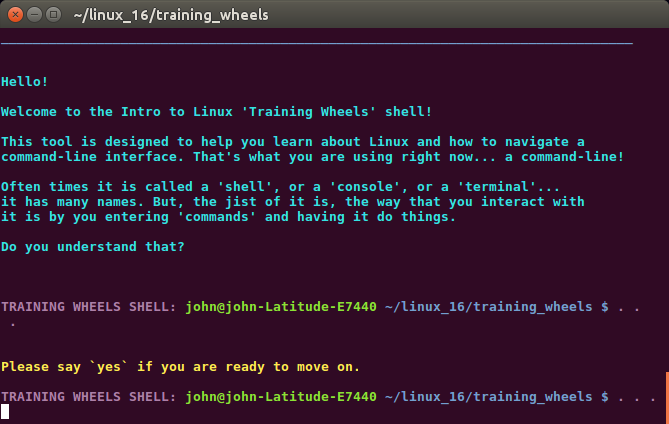
\includegraphics[width=420px,height=300px,keepaspectratio]{training_wheels.png}
		\centering
	\end{center}

	\newpage

	\subsubsection{The Startup Script}

	\begin{lstlisting}[language=Python]
#!/usr/bin/env python
# -*- coding: utf-8 -*-
# @Author: John Hammond
# @Date:   2016-08-24 23:42:10
# @Last Modified by:   John Hammond
# @Last Modified time: 2016-08-28 13:22:13

import readline
import sys
import time
import socket
import os
import subprocess
import textwrap
import threading
import json

try:
	import colorama
except ImportError as e:

	print '''
[!] Error importing colorama! Training Wheels works best with colorama. 
You should be able to install it with the command:
sudo apt-get install python-colorama
'''

	exit(-1)

from shell.wrapper import TrainingWheelsWrapperClass

from colors.colors import *

if ( __name__ == "__main__" ):

	TrainingWheels = TrainingWheelsWrapperClass()

	TrainingWheels.run()
	'''
	# This invokes the Training Wheels shell, which kickstarts the
	# lessons and all the other interactions with the program.
	'''
	\end{lstlisting}	 


	\hrulefill

	\paragraph{} The only dependency that Training Wheels has is the Python module and package called \texttt{colorama}, which is used for displaying color on the command-line.

	\paragraph{} Miraculously, the \texttt{colorama} package is actually installed by default on the full installation of Raspbian.  

	\paragraph{} That is really the only initial test for the wrapper startup script. If the \texttt{colorama} package is not found, the program will complain and exit appropriately. This is what is ran first, when the user invokes the tool from \texttt{./training\_wheels}.

	\paragraph{} You can see I import a lot of modules needed later on in the program, and then
	pass control over to the top-level \texttt{TrainingWheels} object. This object is defined inside of the \texttt{shell} package.

	\subsubsection{The Wrapper Object}

	\paragraph{} The \texttt{shell} package contains the definition for the \texttt{TrainingWheels} object, which acts as the play-pretend shell environment. To simulate a real bash environment, the Training Wheels program only ``fakes'' it. It reads in the user's input, sends it to the system, and returns whatever the system returns.  

	\paragraph{}

	\begin{lstlisting}[language=Python]
# -*- coding: utf-8 -*-
# @Author: John Hammond
# @Date:   2016-08-24 23:44:30
# @Last Modified by:   John Hammond
# @Last Modified time: 2016-08-25 08:56:38

import os
from colors.colors import *
from shell import TrainingWheelsShellClass

class TrainingWheelsWrapperClass():

	def __init__( self ):
		
		os.system("clear")
		print 	B("_" * 79 + "\n\n" ) + c(\
" ... this tool was developed by John Hammond. If you're curious about it, ask!\n"+
			  	B("_" * 79 + "\n\n"))


	def run( self ):

		TraingWheelsShell = TrainingWheelsShellClass()
		TraingWheelsShell.run()
	\end{lstlisting}

	\paragraph{} This code above is just the constructor for the wrapper class. All it does is show a banner that this is \textit{my} software, and then pass control to the real \texttt{TrainingWheelsShell} object.

	\subsubsection{The Shell Object}

	\begin{lstlisting}[language=Python]
# -*- coding: utf-8 -*-
# @Author: John Hammond
# @Date:   2016-08-25 00:02:23
# @Last Modified by:   John Hammond
# @Last Modified time: 2016-10-04 00:19:33

import os
import textwrap
import readline
import colorama
import sys
import socket
import subprocess

from colors.colors import *
from save_engine.save_engine import SaveEngineClass
from lessons.lesson_book import LessonBookClass

class TrainingWheelsShellClass():

	def __init__( self ):

		self.SaveEngine = SaveEngineClass( parent = self )
		self.LessonBook = LessonBookClass( parent = self )

		self.using_time = True
		self.time_on = True

		self.entered_input = ""

		self.commands = {
			"@help" 		: 		self.do_help,		
			"@lessons" 		:	 	self.LessonBook.select_lesson,
			"@concepts" 	:	 	self.LessonBook.select_concept,
		}
		self.special_cases = {
			"quit": self.say_goodbye,
			"cd": self.change_directory,
			"nano": self.protect_from_nano,
			"sudo passwd guest": self.change_guest_password,
		}
	\end{lstlisting}

	\paragraph{} The \texttt{TrainingWheelsShell} is the ``main loop'' of the program. It is the real brain that handles the actual processing of commands and input that the user gives Training Wheels. 

	\paragraph{} This class is large and does not fit all on one page, so I will try to break it down into its smaller functions, which should give me an opportunity to further explain what each function does and why it does it.

	\paragraph{} The constructor, shown above, creates two private variables which are other objects used specifically within Training Wheels. The \texttt{SaveEngine} is the module that I wrote to keep track of saving a users' progress, and the \texttt{LessonBook} is the controller for the ``pages of the textbook,'' which are loaded from external files. I will go into more detail on these objects when we reach their source code.

	\paragraph{} The other boolean variables I declare, \texttt{using\_time} and \texttt{time\_on}, are used for controlling the gradual output of the Training Wheels shell. As a nicety and just to make the teaching tool a bit more user-friendly, it ``types out'' all the output it gives to you that are not command output. This creates more of a dialogue and conversation between me, the content-creator and teacher, and the user on the other end of the screen.

	\paragraph{} \texttt{entered\_input} is a string variable that I use to keep track of what the end-user has actually entered so far. It is just declared here so it knows to act as private variable.

	\paragraph{} The \texttt{commands} dictionary is used to associate commands specific to the Training Wheels shell and their appropriate function callbacks. You will see these functions like \texttt{do\_help} and the like below.

	\paragraph{} The \texttt{special\_cases} dictionary is for exceptions; when a typical bash command does not have the intended behavior, or does not play nicely with Training Wheels by default. It has the same design architecture as the \texttt{commands} dictionary; just the command string associated with the corresponding function call. Examples of this are commands like \texttt{quit}, which should obviously exit the program, or \texttt{cd}, for ``change directory.'' Interestingly enough, because the \texttt{cd} command is a \textit{built-in} for the bash shell, it is not a real binary that is called like others... so we have to essentially build it it ourselves.

	\paragraph{} And I throw in a couple other guards for running things that require line buffering, like \texttt{nano}. Since Training Wheels is meant to be a procedural, line-by-line progression of commands, line-buffering and tools that take advantage of \texttt{ncurses} functionality cause it to explode.

	\paragraph{}

	\hrulefill

	\paragraph{} As stated above, I will try to showcase and explain some of the smaller functions for the class below. In the source code, these routines are not \textit{thoroughly} commented -- \textbf{because rather than striving to comment absolutely every line of source code, you should strive to write readable code in the first place.}

	\subsubsection{General Shell Functions}

	\begin{lstlisting}[language=Python]
	
	def change_guest_password(self):
		# Have to run it this way so the line handling happens correctly...
		os.system("sudo passwd guest")

	def protect_from_nano(self):
		print R("Training Wheels cannot handle running nano!")
		print R("The line buffering causes it to choke... sorry!")

	def change_directory( self ):

		to_directory = " ".join( self.entered_input.split(" ")[1:] )
		to_directory = to_directory.replace("~", os.environ['HOME'] )

		if ( to_directory == '' ):
			os.chdir(os.environ['HOME'])
			
		else:
			try:
				os.chdir(to_directory)
			except OSError:
				print "bash: cd: " + to_directory + ": No such file or directory"

	def do_help( self ):

		print \
		textwrap.dedent('''
	@help:		View this help message.
	@lessons:	Select from a menu of lessons what to study from.
	@concepts:	Choose a concept from the lesson that you are on.
		''' )
	\end{lstlisting}

	\paragraph{} These few functions are the ones that correspond to the some of the above \texttt{commands} and \texttt{special\_cases} dictionaries. They are simple guards to protect the shell from breaking, or offering other necessary functionality. Obviously you can add and remove as many of these as you may need.

	\paragraph{} The really only interesting bit of code here is the \texttt{change\_directory} function. It reads the entered input, snags the arguments out of the command, and moves the program's current working directory to that path.  It accounts for the \texttt{\~} tidle symbol being the short-hand notation for a user's home directory, in case that is present. If no arguments are given, it moves to the user's home directory (based off of the environment variable), just like the usual \texttt{cd} command. If it does not see the path, it spits out the generic error message as you would normally see.

	\subsubsection{Processing the User's Commands}

\begin{lstlisting}[language=Python]
	def process( self ):

		if self.entered_input == "": return

		command = self.entered_input.split(" ")[0]
		# Run the corresponding function in the dictionary
		if command in self.special_cases.iterkeys():
			self.special_cases[command]()
			return True
		if self.entered_input in self.commands.iterkeys():
			self.commands[self.entered_input]()
			raise KeyboardInterrupt
		
		''' If they actually entered something, treat it as a command '''
		try:
			p = subprocess.Popen(	#self.entered_input.split(), 
									self.entered_input, 
									shell = True,
									stdout = subprocess.PIPE, 
									stdin=subprocess.PIPE,
								)

			while ( p ):
				try:
					sys.stdout.write( self.LessonBook.something_to_say_inbetween )
					sys.stdout.write( p.stdout.next() )
				except StopIteration:
					break

		except OSError as e:
			print self.entered_input + ": command not found"

\end{lstlisting}

	\paragraph{}

	\paragraph{} This \texttt{process} function is the core of the \texttt{TrainingWheelsShell} object. It is what creates a new process for the users input, grabs the output, and spits it out on the screen.

	\paragraph{} It starts by testing whether or not the command is in any of our exception dictionaries. If it is, it runs those functions instead, and returns to move on to continue code execution. If it is not, it runs the command in a real shell, and captures the output. It then loops through the output and displays it to the user, adding any in-between text we specify as part of the lesson. And of course, if the command is not a real command, it peacefully throws an error, just like a normal bash shell.

	\subsubsection{The Shell Run Function}

	\begin{lstlisting}[language=Python]
	def error( self, e ):
		print colorama.Back.BLACK + R("Oh no! I hit an error!")
		print r("\n" + str(e.__repr__())), colorama.Back.NC
		print r("\n" + e.child_traceback), colorama.Back.NC

	def run( self ):
		''' The main loop of the program is here, creating the shell...'''

		if (not self.SaveEngine.load() ):

			self.LessonBook.select_lesson()
			self.LessonBook.select_concept()

		while ( True ):

			try:
				
				self.LessonBook.go()

			except KeyboardInterrupt:
				self.time_on = False
				sys.stdout.write("^C\n")
				continue

			except Exception as e:
				self.error(e)
	\end{lstlisting}

	\paragraph{}

	\paragraph{} I would hope at this you see my architecture trickles down by running the corresponding \texttt{run} function for each object I create in my OOP design. 

	\paragraph{} For the \texttt{TrainingWheelsShell} object, it checks the \texttt{SaveEngine} to see if there is any previously saved data that it can load. If there is, it loads it; if not, it offers the user a prompt within the \texttt{LessonBook} object to choose a specific lesson and concept.

	\paragraph{} After a lesson has been chosen, it begins the loop of the program. This is just another pass of control to the \texttt{LessonBook} object, which really controls the users' progress through any lesson in Training Wheels. I also test for \texttt{KeyboardInterrupt}s, like the user pressing \texttt{Ctrl+C}. To really convince the user that they are inside of a shell, I trap them and print out fake ``\^{}C'' strings, like you would normally see in bash. Any other errors are actually unintentional, and lead to formal vomit. Ideally, that \texttt{error} function will never be called.

	\newpage

	\subsubsection{The Save Engine}

	\begin{lstlisting}[language=Python]
# -*- coding: utf-8 -*-
# @Author: John Hammond
# @Date:   2016-08-25 00:29:22
# @Last Modified by:   John Hammond
# @Last Modified time: 2016-09-07 22:19:23

import json
import base64
import os
from colors.colors import *

class SaveEngineClass():

	def __init__( self, parent ):

		self.save_filename = '/tmp/training_wheels.log'
		self.loaded_data = None
		self.parent = parent
		

		if ( os.path.exists( self.save_filename ) ):
			self.save_handle = open( self.save_filename, 'r' )
		else:
			self.save_handle = open( self.save_filename, 'w' )

	def __del__( self ):
		self.save_handle.close()

	\end{lstlisting}

	\paragraph{}

	\paragraph{} The \texttt{SaveEngine} is another object and class that I utilize in Training Wheels. This is the controller for managing the user's saved progress, allowing for functionality to save and load where they have been before.

	\paragraph{} Again, this is a large class that cannot be shown on a single page, so I will showcase functions separately. 

	\paragraph{} Shown above is the constructor and deconstructor for the class. The \texttt{SaveEngine} saves the end-users progress in a static path \texttt{/tmp/training\_wheels.log}, obfuscating it by base64 encoding a JSON dump of data. The constructor just creates a handle object for the file, and the deconstructur just closes it, as necessary.

	\newpage

	\subsubsection{Loading User Data}

\begin{lstlisting}[language=Python]
	def load( self ):
		if ( self.save_handle.closed ):
			self.save_handle = open( self.save_filename, 'r' )

		if ( self.save_handle.mode != 'r' ):
			self.save_handle.close()
			self.save_handle = open( self.save_filename, 'r' )

		try:
			self.loaded_data = json.loads( base64.b64decode( 
												 self.save_handle.read() ) )
		except ValueError:
			return False
			
		if self.loaded_data != {}:

			print M('''
It looks like you've used this tool before! I'll bring you right back to where 
you left off. If you'd like to revisit older lesson or concepts, enter `@help`!''')

			self.parent.LessonBook.load_lesson( self.loaded_data["current_lesson"] )
			self.parent.LessonBook.lesson_pointer = self.loaded_data["lesson_pointer"]
			self.parent.LessonBook.new_lesson_pointer = self.loaded_data["lesson_pointer"]

			return True

\end{lstlisting}

	\paragraph{}

	\paragraph{} The \texttt{load} function will return a boolean \texttt{True} or \texttt{False} depending on whether or not the engine was able to load some previous data.

	\paragraph{} It simply tests if the handle is open, and acts accordingly. It then deobfuscates the loaded data and savess it into a variable that we can pull the JSON data out of.  

	\newpage

	\subsubsection{Saving User Data}

\begin{lstlisting}[language=Python]
	def save( self, data ):
		if ( self.save_handle.closed ):
			self.save_handle = open( self.save_filename, 'w' )

		if ( self.save_handle.mode != 'w' ):
			self.save_handle.close()
			self.save_handle = open( self.save_filename, 'w' )

		self.save_handle.seek(0)
		self.save_handle.write( base64.b64encode( json.dumps( data ) ) )

\end{lstlisting}

	\paragraph{}

	\paragraph{} The \texttt{save} function acts very similarly to the load function, by testing whether or not the file handle is open, and then just writing the obfuscated data passed into the function.

	\paragraph{} This function is called within the \texttt{LessonBook} object, which keeps track of all the necessary data (lesson indices) and then gives it to the \texttt{SaveEngine} as a JSON object.

	\paragraph{} \paragraph{}

	\hrulefill

	\paragraph{} \paragraph{}

	\begin{center}
		\graphicspath{ {.} }
		
\includegraphics[width=200px,height=200px,keepaspectratio]{bash.png}
		\centering
		\vfill
	\end{center}

	\newpage

	\subsubsection{The LessonBook Package}

	\begin{lstlisting}[language=Python]
# -*- coding: utf-8 -*-
# @Author: John Hammond
# @Date:   2016-08-25 00:50:06
# @Last Modified by:   John Hammond
# @Last Modified time: 2016-10-04 00:59:00

import json
from colors.colors import *
import glob
import sys
import textwrap
import time
import curses
import os

class LessonBookClass(object):

	def __init__( self, parent, filename = "" ):

		self.parent = parent
		self.punction_stops = "\n.,!?-"

		path = os.path.dirname(os.path.realpath(__file__))

		self.lesson_pointer = 0
		self.new_lesson_pointer = 0
		self.lesson_is_loaded = False
		self.selected_lesson_number = 0

		self.current_lesson = {}

		self.available_lessons = [file for file in 
					sorted(glob.glob(os.path.join(path, '.*.json')))]

		self.cleaned_available_lessons = [ 	

			l.split('/')[-1][1:].replace('.json','').\
							replace('lesson_','').\
							replace('_',' ')

			for l in self.available_lessons  ]

		self.seen_entries = {}
		self.something_to_say_inbetween = ""

		
\end{lstlisting}

	\paragraph{}

	\hrulefill

	\paragraph{} The \texttt{LessonBook} object is really what drives the idea of "progress" within Training Wheels. It is what acts as the story, or the ``interactive textbook''.

	\paragraph{} This class is actually the largest of all of the objects within Training Wheels, so I think it should go without saying that the source code will spread across multiple pages. 

	\paragraph{} Shown above is the constructor for the class. The object keeps track of its parent (which is the \texttt{TrainingWheelsShell} as you have seen in the previous code) for easy handling. The variable \texttt{punctuation\_stops} is used for timing; the ``type-out'' effect pauses for just a little while longer on actual grammatical pauses.

	\paragraph{} This constructor initializes some private variables that I use to keep track of the users' \textit{position} within a lesson. The ``lesson'' is just a giant array or list, and the ``pointer'' is a just a number indicating what index they are on.

	\paragraph{} I use the Python \texttt{glob} module to look in this directory to find any lesson files, which are really just JSON configurations. The title of the lesson is actually formatted by the filename, so I scrape the name and clean it up with some string replace methods.

	\subsubsection{The ``Type-Out'' Effect}

\begin{lstlisting}[language=Python]
	def say( self, message ):

		if ( not message.endswith('\n\n') ): message += '\n\n'

		for character in message:
			sys.stdout.write(character)
			sys.stdout.flush()
			if self.parent.using_time:
				if self.parent.time_on:
					if character in self.punction_stops:
						time.sleep(0.12)
					else:
						time.sleep(0.04)		
\end{lstlisting}

	\paragraph{}

	\paragraph{} Training Wheels achieves it's ``type-out'' effect by the above function. The function is really just a wrapper for a classic \texttt{print} statement, but it checks with the parent (the \texttt{TrainingWheelsShell} object) if it will stagger each character, to creare a visual effect that looks like someone is printing the message by typing on a keyboard. 

	\paragraph{} I check if there are some newlines present just for cleanliness, and then I display each character of the message one by one. You can see the variables \texttt{parent.time\_on} being put to use in the test. I just delay for a small segment of time if they are set to \texttt{True}. 

	\subsubsection{General LessonBook Functions}

	\begin{lstlisting}[language=Python]
	def is_in_directory( self, directory = None ):
		if directory == None: return True
		else: return os.getcwd() == directory.replace("~", os.environ["HOME"])
\end{lstlisting}

	\paragraph{}

	\paragraph{} There is only one small and general function I created just for use within the \texttt{LessonBook} class. I had added some functionality to test if the user is in the right directory, if the ``lesson'' specifies that they need to be a specific one. I use this conditional more than once, so I just put it in a function for cleanliness.

	\subsubsection{Loading a Lesson}

\begin{lstlisting}[language=Python]
	def load_lesson( self, lesson_identifier ):

		try:
			self.file_handle = open(lesson_identifier, 'r')
		except IOError:
			# The file does not exist.
			raise Exception("This file does not exist!")
		
		self.current_lesson = json.loads( self.file_handle.read() )
		self.selected_lesson_number = int(self.current_lesson['name'].split(".")[0]) - 1
		
		self.lesson_is_loaded = True
\end{lstlisting}
	
	\paragraph{}

	\paragraph{} The \texttt{LessonBook} object needs to have functionality to \textit{load a lesson} and set it as the currently running lesson, so this is generalized in the above function. 

	\paragraph{} It just takes a string as an argument which is the real filename of the JSON lesson file. It reads the contents of the file and then JSON processes it into an actual Python dictionary, and we specify the \texttt{selected\_lesson\_number} variable to be the zero-based number of that lesson file.

	\newpage

	\subsubsection{Moving to the next Lesson }

	\begin{lstlisting}[language=Python]
	def go_to_next_lesson( self ):

		print M("It looks like you are all done with this lesson!")
		print M("I'm going to move you to the next one. You are now on lesson:\n")

		next_lesson_number = self.selected_lesson_number + 1

		if ( next_lesson_number >= len( self.available_lessons ) ):
			print( Y("Actually -- there are no more lessons!") )
			print( Y("You're all done for now... go practice Linux!") )
			self.parent.SaveEngine.save( "done" )
			exit()
		else:

			next_lesson_name = self.cleaned_available_lessons[next_lesson_number]
			print "\t" + next_lesson_name + "\n\n"

			self.lesson_pointer = 0
			self.new_lesson_pointer = 0
			self.selected_lesson_number += 1
			self.load_lesson( self.available_lessons[next_lesson_number] )
	\end{lstlisting}

	\paragraph{}

	\paragraph{} When a student has finished a lesson in the lesson book, if there are others to move on to, Training Wheels should automatically move them into it. This is done with the above function. It notifies the user that they completed the lesson, and increments their \texttt{selected\_lesson\_number} variable and counter.

	\paragraph{} You can see in the code that if Training Wheels catches that there are no more lessons, it tells the user that are done for the time being, saves their progress, and ends the program. 

	\paragraph{} Note that if they \textit{do} move on to a new lesson, it resets the counter variables (\texttt{lesson\_pointer} and the like) and loads the new lesson, with the same function you saw previously.

	\newpage

	\subsubsection{Selecting a Lesson }

\begin{lstlisting}[language=Python]
	def select_lesson( self ):

		if ( not self.lesson_is_loaded ):
			print M("\nIt looks like a lesson has not yet been loaded.")
		else:
			print M("\nYou already have ") + C(self.current_lesson["name"]) + M(" loaded.")
			print M("Load something else?")

			entered = False
			while ( not entered ):
				answer = raw_input("(y/n): ").lower()
				if answer == "yes" or answer == "y":
					self.lesson_is_loaded = False
					self.lesson_pointer = 0
					self.new_lesson_pointer = 0
					entered = True
					pass
				elif answer == "no" or answer == "n":
					return
				else:
					print R("\nPlease enter yes or no.")

		print M('''
Please select one of the available lessons by entering the corresponding number.
Enter the number '0' to go back to what you were doing.\n''')		

		for l in self.cleaned_available_lessons:
			print "\t", l
		print "\n\n"

		
	\end{lstlisting}	

	\paragraph{}

	\paragraph{} This \texttt{select\_lesson} function continues onto the following page.

	\newpage

	\begin{lstlisting}[language=Python]

		while ( not self.lesson_is_loaded ):
			print M("lesson #:"),
			self.selected_lesson_number = raw_input()

			if ( self.selected_lesson_number == "0" or self.selected_lesson_number == "quit" ):
				return

			try:
				self.selected_lesson_number = int( self.selected_lesson_number ) - 1
			except:
				print R("That does not look like a valid input. Please try again.")
				continue

			if ( self.selected_lesson_number >= 0 and 
				self.selected_lesson_number < len(self.available_lessons) ):

				print B("_"*79 + "\n")
				self.load_lesson( self.available_lessons[self.selected_lesson_number] )
				
				return
			else:
				print R("That does not look like a valid input. Please try again.")
				continue

	\end{lstlisting}	

	\paragraph{} This classes' \texttt{select\_lesson} is what is first seen by the user when they invoke Training Wheels and have not yet started a lesson. If they \textit{have} already started a lesson, as you can see it will prompt the user to confirm that they really want to load something else. It keeps error-checking their input until they enter a valid yes or no answer.

	\paragraph{} It then prints out all of the available lessons, so the user can see them all displayed. Again, Training Wheels prompts for and ensures valid input, and once a decision has been made it will load the appropriate lesson.


	\newpage 

	\subsubsection{Selecting a Concept}

	\begin{lstlisting}[language=Python]
	def select_concept( self ):
		if ( self.current_lesson == {} ):
			print R("There is currently no lesson loaded!")
			print R("Enter `@lessons` to select one to load.")
			return 

		print M('''
The current lesson that is loaded is: ''') + \
C(self.current_lesson["name"]) + \M('''".
Please select one of the concepts you would like to jump to.
The lesson you are currently looking at is highlighted in '''+\
y('yellow') + M(".Enter the number '0' to go back to what you were doing.\n"))

		# Display all of the concepts that are available.
		for i in range( len(self.current_lesson["concepts"]) ):
			number = str(i + 1)
			if i == self.lesson_pointer:
				print "\t" + Y( number + ". " +self.current_lesson["concepts"][i]["tag"])
			else:
				print "\t" + number + ". " + self.current_lesson["concepts"][i]["tag"]
		print "\n\n"
		
		selected = False	
	\end{lstlisting}	

	\paragraph{}

	\paragraph{} This \texttt{select\_concept} function continues on to the following page.

	\newpage

	\begin{lstlisting}[language=Python]
		while ( not selected ):
			print M("concept #:"),
			selected_concept_number = raw_input()

			if ( selected_concept_number == "0" or selected_concept_number == "quit" ):
				return
			try:
				selected_concept_number = int( selected_concept_number ) - 1
			except:
				print R("That does not look like a valid input. Please try again.")
				continue

			if ( selected_concept_number >= 0 and 
				selected_concept_number < len(self.current_lesson["concepts"]) ):

				self.lesson_pointer = selected_concept_number
				self.new_lesson_pointer = selected_concept_number
				print B("_"*79 + "\n")
				return
			else:
				print R("That does not look like a valid input. Please try again.")
				continue
	\end{lstlisting}

	\paragraph{} The \texttt{select\_concept} function is what is presented to the user after choosing a lesson. The function looks into the selected lesson (if one is present; if not, it returns) and displays each ``concept'' out to the screen.

	\paragraph{} This is typically a large amount of output, so the user will may have to scroll through it.

	\paragraph{} Each ``concept'' is really just each \textit{question}, or unique \textit{prompt} as you progress through a lesson in Training Wheels. I just offer this functionality so the user may not have to re-work through an entire lesson; if they want to, they can jump to any point in the lesson.

	\paragraph{} The user can, of course, invoke this selection screen at anytime by entering one of the special case commands, \texttt{@concepts}.

	\newpage

	\subsubsection{The Main Loop}

	\begin{lstlisting}[language=Python]
		def go( self ):
			# This function is too large to be shown in the text
	\end{lstlisting}


	\paragraph{} The \texttt{go} function of the \texttt{LessonBook} object, and ultimately the core loop of the entire Training Wheels program, is so large that it covers not just more than two pages here; it covers four.

	\paragraph{} For that reason I chose not to include it here. The function can be seen and accessed in the github repository under the \texttt{training\_wheels} directory and in the \texttt{lesson\_book.py} Python code of the \texttt{lesson} package.

	\paragraph{} The function is so large because it does so many things. Without showing code, I will still try and at least list what it does:

	\begin{enumerate}
		\item Save the current position in the running lesson
		\item Retrieve all the properties for the current concept (the message prompt, the hint, the correct command, the necessary directory, etc.)
		\item Display the message prompt for the process and wait for user input
		\item Split up and parse the input to determine the command and arguments
		\item Check if the user is in the necessary directory
		\item Process the command and their input
		\item Increment the pointer to progress them through the lesson
	\end{enumerate} 

	\paragraph{} I have said before that the \texttt{TrainingWheelsShell} object is the brain that handles commands and processing their output and behavior. In that sense, it is instead the \texttt{LessonBook} object and the \texttt{go} function that is the brain that handles whether or not the user \textit{progresses} through the content and material of Training Wheels. 

	\newpage

	\subsection{The JSON Lessons}

	\paragraph{} You, as the future instructor or the inheritor of all of this, are probably not so interested in the source code of Training Wheels, but instead, the lessons that it can offer. If you really wanted to go under the hood and change the way that Training Wheels worked or had to fix or bug or something, you could dive into the code... but you would have to know the Python programming language.

	\paragraph{} To create \textit{content} for Training Wheels on the other hand, the only other language you need to know is English.

	\subsubsection{Using HJSON}

	\paragraph{} All of the lessons for Training Wheels are JSON objects; but, for development purposes, they first \textit{start out} as HJSON.

	\paragraph{} If you have never heard of HJSON, that's okay. It is named: ``Human-Readable''-JSON, in that it adds a lot of syntactic sugar and niceties. 

	\paragraph{} You should check out the HJSON project online for a more formal grasp on it (\href{https://hjson.org/}{https://hjson.org/}), but here are some of the cool things it offers:

	\begin{itemize}
		\item Trailing commas are optional for data fields
		\item Support for different kinds and styles for commenting (\texttt{\#}, \texttt{\/\/}, etc.)
		\item You can specify strings without quotes (``'' )
		\item \textbf{Support for multi-line strings}
	\end{itemize}

	\paragraph{} The last one, support for multi-line strings, is really \textit{really} big for us.

	\paragraph{} Because we are writing large prompts and should be explaining lots of in-depth concepts, we really need easy and simple support for our multi-line strings.

	\paragraph{} So, I initially wrote all of the lesson files in HJSON ... but Python doesn't know how to process and import HJSON all that easily (and I wasn't going to write a custom parser for this project, as well, sorry). That means that if we use HJSON we have to convert it all back into JSON.

	\paragraph{} You can do this very easily with the command-line \texttt{hjson} utility, and I did it so often I ended up just cooking a small script to run through and convert \textit{all} of the lesson files.

	\paragraph{} As the developer, you can do this with the \texttt{hjson} utility, too. But first you need to get it. Thankfully, I wrote some setup code for Training Wheels, so you can be on your feet and running in no time.

	\subsubsection{Getting HJSON} 

	\begin{lstlisting}[language=Bash]
#!/bin/bash
# @Author: John Hammond
# @Date:   2016-08-28 15:08:22

BLACK=`tput setaf 0`;RED=`tput setaf 1`;GREEN=`tput setaf 2`
YELLOW=`tput setaf 3`;BLUE=`tput setaf 6`;NC=`tput sgr0`

DEPENDENCIES="nodejs-legacy npm"

function install_dependencies(){

	echo "${FUNCNAME}:${GREEN} installing nodejs and npm...${NC}"
	apt-get -y install $DEPENDENCIES || fatal_error
}

function install_hjson(){

	echo "${FUNCNAME}:${GREEN} installing hjson with npm...${NC}"
	npm install hjson -g
}

function fatal_error(){
	echo "${FUNCNAME}:${RED} aborting...${NC}"
	exit -1
}

function main(){
	echo "${BLUE} This script will install the dependencies that you should have"
	echo "${BLUE} to develop for the Training Wheels shell."
	echo -e "${BLUE} It is really just for convenience sake of using HJSON.\n ${NC}"

	install_dependencies
	install_hjson
}

if [ "$UID" != "0" ]
then
	echo "You must be root to run this script!"
	fatal_error
fi

main $@
	\end{lstlisting}


	\newpage

	\paragraph{} HJSON is apparently written in JavaScript, so you can run it with Node.js. 

	\paragraph{} This bash script will install Node.js and \texttt{npm}, the Node Package Manager. From there it has \texttt{npm} install the HJSON package. Once the script is done, you should have \texttt{hjson} in your \texttt{PATH}, which you can use to convert any file.

	\paragraph{} Honestly, this script could be boiled down into two lines:

	\begin{lstlisting}[language=Bash]
sudo apt-get -y install nodejs-legacy npm
npm install hjson -g
\end{lstlisting}

	\paragraph{} ... But, for good packaging, the fully-fleshed out and user-friendly setup script is given.

	\subsubsection{Converting HJSON to JSON}

	\paragraph{} Because this is such a common thing, I made it a practice to store the HJSON files in the lessons package directory, and run a script to convert them all into hidden JSON files. On the repository, this is is the \texttt{compile\_lessons.sh} script.

	\begin{lstlisting}[language=Bash]
#!/bin/bash

ls *.hjson|while read line; do hjson -j "$line" > ".${line/hjson/json}"; done

# We should add in a carriage return to all new-lines so we can
# use the curses mode!
ls .*.json|while read line
do
	sed -i 's/\\n/\\n\\r/g' ${line}
done
\end{lstlisting}	

	\paragraph{} The script is honestly just a one-liner while loop, with some bash variable string replacement for convenience. It was just contained in a \texttt{compile\_lessons.sh} script so I (and you as the developer) don't have to type that out all the time.

	\paragraph{} If you ever do write new lessons for Training Wheels, \textbf{DO NOT FORGET TO DO THIS}. Training Wheels will only look for \texttt{.json} files, so if you have not convered your lesson, when you run training Wheels, it will look like it is not there at all!

	\paragraph{} As you can see in the above script, it only runs \texttt{ls *.hjson} in the current directory, so for the script to actually do something, you must run it inside the \texttt{lessons} package and directory.

	\newpage

	\subsubsection{HJSON Lesson File Syntax}

	\paragraph{} You can find all of the HJSON and JSON lesson files in the \texttt{lesson} package and directory of the github repository, but as an example, here is some sample syntax:


	\begin{lstlisting}[language=Bash]
{
  "name" : "7. Working with Files",
# =============================================================

  "concepts": [

  {
    
"tag" : "Let's start at the temporary directory",

"message" : '''

Let's start to work with some files. Please move to the temporary directory so
we have a place to work.

  ''',

"command_waiting" : "cd /tmp",

"incorrect":"Do you remember how to `cd` to the temp directory?",

  },

# -------------------------------------------------------------

\end{lstlisting}	

	\paragraph{} The outermost object is the lesson itself, with a \texttt{name} variable being set to the lesson number and title.

	\paragraph{} Inside of it is the \texttt{concepts} array, which houses a ton of other objects, each with a property for a \texttt{tag}, \texttt{message}, \texttt{command\_waiting}, and \texttt{incorrect}.

	\paragraph{} In a \texttt{concept} you can also specify a \texttt{proper\_directory} variable, which you can set to a path that the user should be in for that specific prompt.

	\newpage

	\subsection{Your Mileage May Vary}

	\paragraph{} After the Fall 2016 rendition of Intro to Linux, I had written about ten separate lessons within Training Wheels. They are as follows:

	\begin{enumerate}
		\item Welcome to Training Wheels
		\item The Man Pages
		\item Your Home Directory
		\item Absolute and Relative Paths
		\item Paths and Files
		\item Special Places and Catting Files
		\item Working with Files
		\item Filters and Pipes
		\item Users Root and Sudo
		\item Adding and Removing Users
	\end{enumerate}

	\paragraph{} Please keep in mind that this is not the end-all be-all of the Linux class, or of my software. This is not the most elegant program, with not the most elegant lessons, and not the most elegant documentation.

	\paragraph{} However, once I am long and gone, it becomes your responsibility to do with it what you will. So, I remind you: \textbf{your mileage may vary}. Hopefully, you can tweak and customize the product to your liking.

	\paragraph{} When I was speaking with LCDR Wyman one day, I had jokingly said that ``Training Wheels'' needed a cool and quick name, just like what \textbf{bash} has. The name ``bash'' comes from \textbf{B}ourne-\textbf{A}gain \textbf{Sh}ell, so I wanted something fancy for my \textbf{Tra}ining Wheels \textbf{Sh}ell. 

	\paragraph{} With that, I give you:  \textbf{\textit{trash}}.

	\newpage


	\section{The Scavenger Hunt}

	\paragraph{} The Scavenger Hunt was designed to be more of a fun and engaging exercise, to let the students put to use what they had learned in the early lessons of Training Wheels.

	\paragraph{} This activity followed after the lesson on the Linux filesystem, after the students learned how to navigate the file structure and how to \texttt{cat} and display files. It was very elementary and simple, but I think it really reinforced how to move and navigate around the file system; and they get to explore Linux all along the way.


	\begin{center}
		\graphicspath{ {.} }
		\makebox[\textwidth]{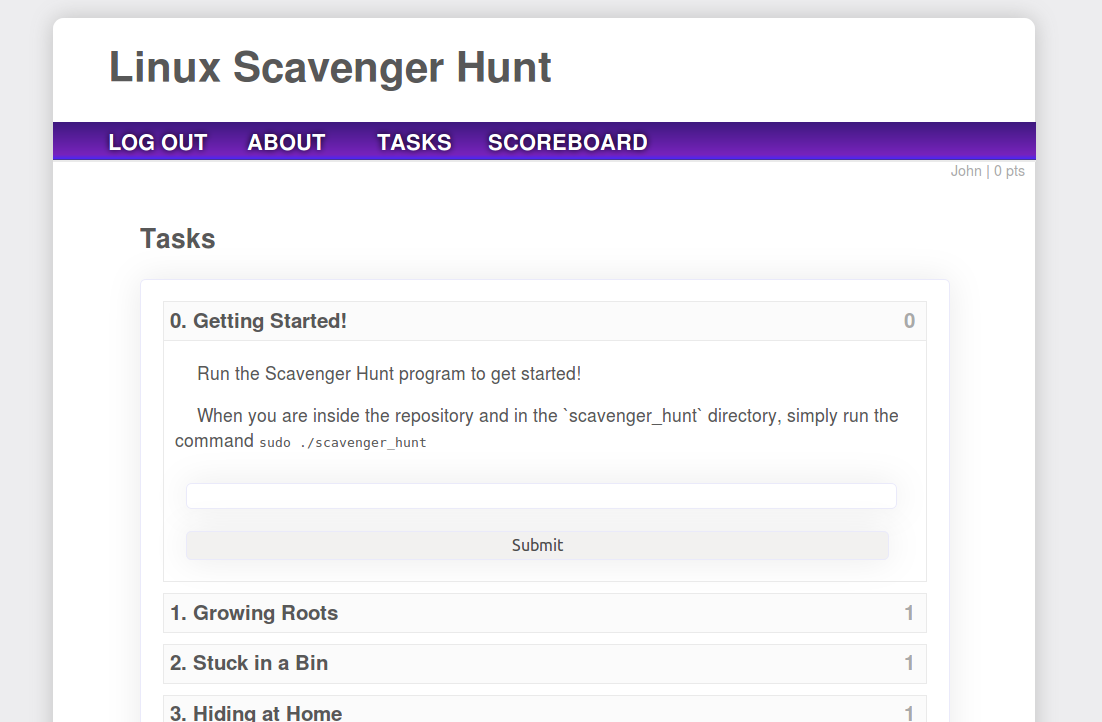
\includegraphics[width=500px,keepaspectratio]{scavenger_hunt.png}}
		\centering
	\end{center}


	\subsection{Conceptual Design}

	\paragraph{} The idea behind the Linux Scavenger Hunt was very much like a cybersecurity competition, or a Capture-the-Flag (CTF) game. Each student was a player, and they would solve problems and answer questions in a Jeopardy-style manner, and the points they earned were visible on the scoreboard.

	\paragraph{} The hope was that it would let the students demonstrate and apply what they have learned, and work with a bit of a competitive-edge. Also, it is a good benchmark as an instructor; you can view the scoreboard and see who was solved what challenges or what amount of progress have they made.


	\subsection{Technical Design}

	\paragraph{} While I said that the Scavenger Hunt was to emulate a CTF, the software that it was built off of was actually the CTF platform that I wrote for the US Coast Guard Academy Cyber Team. 

	\paragraph{} The server is written in Python, using the Flask web microframework. Flask uses Jinja2 for HTML templating. The ``challenges'' or ``tasks'' are stored in a separate JSON file (for extensibility). 

	\paragraph{} The client-side browser experience is just your typical HTML, CSS and JavaScript recipe. I use a bit of jQuery to make some pretty animations and ultimately try to create a simple but aesthetic design.

	\paragraph{} On the server-side, there are lots of different files that you as the developer need to be aware of.

	\subsection{The Database Schema}

	\begin{lstlisting}[language=sql]
drop table if exists users;
create table users (
  id integer primary key autoincrement,
  username text not null,
  password text not null,
  solved_challenges text not null,
  score integer not null,
  last_submission integer not null
);
\end{lstlisting}	

	\paragraph{} There is a backend database, built in SQLite3, that really just keeps track of the users. 

	\paragraph{} Obviously it needs to keep track of their username, their password hash (the server stores a SHA256 hash), the challenges that they have solved, their score, and the time of their last submission (in case of a tie in points).

\subsection{The Clean Script}

	\begin{lstlisting}[language=bash]
#!/bin/bash

rm -f server.py certificate.crt privateKey.key
\end{lstlisting}	


	\paragraph{} The server creates and signs its own certificate, so it can send encrypted traffic with HTTPS. The certificate is generated with the setup script, along with a properly configured version of the server. 

	\paragraph{} For convenience, there is just a simple \texttt{clean.sh} script that removes these files. They can always be regenerated with the \texttt{setup.sh} script.


	\newpage

	\subsection{The Setup Script }

	\begin{lstlisting}[language=bash]
#!/usr/bin/env bash
# Author: John Hammond
# Date: 11JAN2016
# Description:
# This script should install all dependencies & generate a 
# self-signing certificate to be used by a CTF server you can 
# run on your own local machine. If you configure your own CTF 
# with a .json file, you can give that to the server script 
# and it will easily spin up a CTF competition for everyone 
# in the local network.

# Optional: should be modified by the cmd-line arguments
DATABASE=""
CONFIGURATION=""

# Internal variables; do not edit.
DEPENDENCIES="python-pip sqlite3 python-flask python-passlib"
SERVER_FILE="server_base.py"
NEW_SERVER_FILE="server.py"
SCHEMA_FILE="schema.sql"
PRIVATEKEY_FILE='privateKey.key'
CERTIFICATE_FILE='certificate.crt'

CURRENT_USER=`logname`
RED=`tput setaf 1`;GREEN=`tput setaf 2`;NC=`tput sgr0`

function display_help() {
	cat <<EOF
usage:
	$0 -d DATABASE -c CONFIGURATION
parameters:
	-d
		Specify the database file that will be created and used for this server.
		Example: '/tmp/ctf-practice.db'
	-c
		Specify the configuration file that will be used for this server.
		Example: 'ctf_practice.json'
	-h
		Display help message
EOF
}
\end{lstlisting}

	\paragraph{} This \texttt{setup.sh} script continues on to the next page.

	\newpage

		\begin{lstlisting}[language=bash]
function create_new_server(){

	cp $SERVER_FILE $NEW_SERVER_FILE
	chown $CURRENT_USER $NEW_SERVER_FILE
	chmod 744 $NEW_SERVER_FILE
}

function configure_firewall(){
	
	# Allow incoming connections...
	echo "$0: ${GREEN} Configuring firewall for HTTPS connections...${NC}"
	ufw allow https
}

function main()
{

	install_dependencies
	create_new_server
	create_certificate
	create_database
	configure_ctf
	configure_firewall

	echo "$0: ${GREEN} CTF server successfully setup!${NC}"
	echo "$0: ${GREEN} You should now be able to run the server with the command: ${NC}"
	echo '`sudo python server.py`'

	exit 0
	
}

main "$@"
\end{lstlisting}

	\paragraph{} There are many other functions and lines of code that I have omitted here; but the \texttt{main} function does a good job of listing what the code does.

	\paragraph{} There are many other functions, like \texttt{create\_database}, \texttt{create\_certificate},  \texttt{configure\_ctf}, and others that really just use \texttt{sed} to do some replacing in the original server script, to configure and create a whole new server script.

	\paragraph{} As stated above, the \texttt{setup.sh} script will spit out a new \texttt{server.py} file that you are intended to run as your server.

	\newpage

	\subsection{The Backend Server Source Code}

	\paragraph{} The server is all one in file, actually; it is nowhere near as broken down and organized as Training Wheels is.

	\subsubsection{Importing the Modules}

\begin{lstlisting}[language=Python]
#!/usr/bin/env python

from flask import Flask
from flask import render_template, request, session, g, url_for, flash, get_flashed_messages, redirect
import sqlite3
import json
import sys, os
from colorama import *
import sys

from passlib.hash import sha256_crypt
from contextlib import closing

debug = True
init( autoreset = True )

if (debug):

	def success( string ):
		print Fore.GREEN + Style.BRIGHT + "[+] " + string

	def error( string ):
		sys.stderr.write( Fore.RED + Style.BRIGHT + "[-] " + string + "\n" )

	def warning( string ):
		print Fore.YELLOW + "[!] " + string

else:
	def success( string ): pass
	def error( string ): pass
	def warning( string ): pass
\end{lstlisting}

	\paragraph{} As I said the code is written in Python, and I utilize Flask and JSON and Sqlite, for the web server, configuration files, and database respectively. I also use the Python \texttt{passlib} module for the SHA256 hashing (though I could have just as easily used \texttt{hashlib} and avoided a dependency).

	\paragraph{} For debugging and development purposes I create a couple wrapper functions that just print out messages on the server side in color with the \texttt{colorama} module. These are only set if you decide that \texttt{debug} is on. If not, the functions do nothing.

	\newpage

	\subsubsection{Server Configuration}

\begin{lstlisting}[language=Python]
# ============================================================

DATABASE = '$DATABASE'
CONFIG = '$CONFIGURATION'
CERTIFICATE = '$CERTIFICATE_FILE'
PRIVATE_KEY = '$PRIVATEKEY_FILE'

SECRET_KEY = 'this_key_needs_to_be_used_for_session_variables'

if DATABASE == '$DATABASE':
	error("This server has not yet been configured with a database file!")
	exit(-1)

if CONFIG == '$CONFIGURATION':
	error("This server has not yet been configured with a configuration file!")
	exit(-1)

if CERTIFICATE == '$CERTIFICATE_FILE':
	error("This server has not yet been configured with a certificate!")
	exit(-1)

if PRIVATE_KEY == '$PRIVATEKEY_FILE':
	error("This server has not yet been configured with a private key!")
	exit(-1)

app = Flask( __name__ )

app.config.from_object(__name__)

needed_configurations = [
	"app_title", "app_about", "app_navigation_logged_out",
	"app_navigation_logged_in", "challenges"
]
\end{lstlisting}
	
	\paragraph{} The \texttt{server\_base.py} code has variables that are intentionally meant to be configured by the \texttt{setup.sh} script. These are the \texttt{DATABASE}, \texttt{CONFIG},  \texttt{CERTIFICATE}, and \texttt{PRIVATE\_KEY} variables. These all must be configured, as you can see with the tests.

	\paragraph{} Then, we tell Flask to configure its app within this source code file. Flask needs to do this so it knows things like the database and secret key.

	\newpage

	\subsubsection{Configuration Validation}


\begin{lstlisting}[language=Python]
if not ( os.path.exists(CONFIG) ):
	error("This configuration file '" + CONFIG + "' does not seem to exist!")
	exit(-1)
else:
	success("The configuration file exists!")
	handle = open( CONFIG )
	configuration = json.loads(handle.read().replace("\n","").replace("\t",""))
	try:
		for needed_config in needed_configurations:
			assert configuration[needed_config]
	except Exception as e:	
		error("Configuration file '" + sys.argv[1] + "' does not have the following configuration tag:")
		warning(e.message)
		error("Please fix this and re-run the server.")
		exit(-1)
	
	handle.close()

	success("The configuration looks good!")
	success("Spinning up the server...")
\end{lstlisting}

	\paragraph{} The server will not start without all the properly configured variables, as you saw in the previous segment of code. Even after reading from the external configuration file, it verifies that it has the necessary properties and variables set.

	\paragraph{}


	\begin{center}
		\graphicspath{ {.} }
		\makebox[\textwidth]{
\includegraphics[width=200px, keepaspectratio]{python-logo.png}}
		\centering
	\end{center}
	

	\hrulefill
	
	\newpage


	\subsubsection{Database Boilerplate}

\begin{lstlisting}[language=Python]
def init_db():
	with closing(connect_db()) as db:
	    with app.open_resource(app.config['DATABASE'], mode='r') as f:
	        db.cursor().executescript(f.read())
	    db.commit()

def connect_db():
	return sqlite3.connect( app.config['DATABASE'] )

@app.before_request
def before_request():
    g.db = connect_db()

@app.teardown_request
def teardown_request(exception):
    db = getattr(g, 'db', None)
    if db is not None:
		db.close()
\end{lstlisting}


	\paragraph{} Following the configuration validation I declare some functions necessary for Flask and its communication with the database. This is the typical boilerplate code you see in their documentation and examples, just using a general-purpose database file, which you can see it reads from the configuration object.


	\subsubsection{Template Rendering Wrapper}

\begin{lstlisting}[language=Python]
def render( template_name, **kwargs ):
	return render_template( template_name, 
							app_title = configuration['app_title'], 
							app_navigation_logged_out = configuration['app_navigation_logged_out'],
							app_navigation_logged_in = configuration['app_navigation_logged_in'],
							**kwargs
						  )
\end{lstlisting}


	\paragraph{} Typically in Flask you can render Jinja2 templates with the function \texttt{render\_template}. This allows you to pass in keywords arguments, for variable and value pairs that should be substituted into the template. Since I do this for each page with the navigation links (so they are easily customizable in just one location), I wrapped the typical Flask \texttt{render\_template} method into a more general purpose one. 

	\newpage

	\subsubsection{The Welcome Page}

	\begin{lstlisting}[language=Python]
@app.route("/")
@app.route("/about")
def about(): return render("about.html", app_about=configuration['app_about'])
\end{lstlisting}

	\paragraph{} The first page presented to you for the Linux Scavenger Hunt doubles as the ``About'' page. There is really not much there other than a small blurb as to what the project really is -- but the intention is that the first thing the user should do is move to the registration page.

	\subsubsection{Registration Functionality}

	\begin{lstlisting}[language=Python]
@app.route("/register", methods=["GET", "POST"])
def register():

	cur = g.db.execute('select username from users')
	usernames = [row[0] for row in cur.fetchall() ]

	error = ""
	if request.method == "POST":

		if unicode(request.form['username']) in usernames:
			error = 'This username is already in use!'
		elif (request.form['password'] == ""):
			error = "You must supply a password!"
		elif request.form['password'] != request.form['confirm']:
			error = 'Your passwords do not match!'
		else:

			cur = g.db.execute('INSERT INTO users (username, password, solved_challenges, score, last_submission) VALUES ( ?, ?, ?, ?, ? )', [ 
				               request.form['username'], 
				               sha256_crypt.encrypt( request.form['password']),
				               "",  # No challenges completed
				               0,   # no score.
				               0,   # and no last submission time.
				  ] )

			g.db.commit()

			flash("Hello " + request.form['username'] + ", you have successfully registered!")
			session_login( request.form['username'] )
			return redirect( "challenges" )

	return render( 'register.html', error = error )
\end{lstlisting}

	\paragraph{} The code above is what allows for the user to create an account and begin to play the game. If the user \texttt{POST}s to the website with a username and password, it checks if the username is not already in the database (and the typical password checks). If everything checks out, it executes the classic SQL instruction to insert the new user.

	\paragraph{} Note that I hash their password with SHA256, and I initialize everything to zero. No solved challenges, no score, and no last submission time. They should be a completely new user.

	\paragraph{} Then I notify them that they have successfully signed up, and I throw them towards the challenges page so they can start the exercise.

	\subsubsection{Login Functionality}

	\begin{lstlisting}[language=Python]
@app.route("/login", methods=["GET", "POST"])
def login():

	error = ""
	if request.method == "POST":

		cur = g.db.execute('select username, password from users')
		users = dict(( row[0], row[1] ) for row in cur.fetchall())

		if not request.form['username'] in users.iterkeys():
			error = 'This username is not in the database!'
		else:
			if not ( sha256_crypt.verify( request.form['password'], users[request.form['username']] ) ):
				error = "Incorrect password!"
			else:
				
				session_login( request.form['username'] )
				return redirect( "challenges" )

	return render( 'login.html', error = error )
\end{lstlisting}

	\paragraph{} If the user already has an account and they just need to login, this code handles their submission. As usual, they \texttt{POST} to the website with their username and password. If their username exists in the database and the hash of their password matches what is found in the database, they are successfully logged in.

	\paragraph{} If they aren't \texttt{POST}ing to the page, we just render out the login page for them so they have a form to work with. 

	\paragraph{} Note that for the actual process of logging in, I accomplish this with another function I've created called \texttt{session\_login}.


	\newpage

	\subsubsection{Session Handling for Logins}

	\begin{lstlisting}[language=Python]
def session_login( username ):
	
	flash("You were successfully logged in!")

	cur = g.db.execute('select solved_challenges, score from users where username = (?)',
			[username])	

	solved_challenges, score = cur.fetchone()

	session['logged_in'] = True
	session['username'] = username
	session['solved_challenges'], session['score'] = solved_challenges, score

def session_logout():

	flash("You have been  successfully logged out.")

	session['logged_in'] = False
	session.pop('username')
	session.pop('score')

\end{lstlisting}

	\paragraph{} Note that these functions do not have a Python decorator, like some of the others you have seen. The decorator is what helps Flask determine what page or URL that this function refers to --- but since these are low-level and general-purpose functions, they should \textit{not} be treated as Flask web pages and therefore do \textit{not} have the decorator. 
	\paragraph{} All these functions particularly do is manage the session variables that I use to consider whether or not the user is ``logged in'', and to keep track of information that I need to share between pages (like their score or the challenges they have solved).

	\paragraph{} The \texttt{session\_login} function takes in the username (which is assumingly passed in by the \texttt{login} function), pulls down their score and solved challenges from the database, and just stores them in the session. The \texttt{session\_logout} function just removes them.

	\paragraph{}


	\begin{center}
		\graphicspath{ {.} }
		\makebox[\textwidth]{
\includegraphics[width=200px, keepaspectratio]{flask.png}}
		\centering
	\end{center}
	
	\newpage


	\subsubsection{The Scoreboard}

	\begin{lstlisting}[language=Python]
@app.route("/scoreboard")
def scoreboard(): 

	cur = g.db.execute('SELECT username, score FROM users ORDER BY score DESC, last_submission ASC')	
	response = cur.fetchall()	
	
	users = [ { "username": row[0], "score": row[1] } for row in response]
	
	return render("scoreboard.html", users = users )

@app.route("/logout")
def logout():

	session_logout()
	return redirect("about")

@app.route("/challenges")
def challenges_page(): 
	if not ( session['logged_in'] ):
		return render("login.html", error = "You must log in to be able to see the challenges!")	
	return render("challenges.html", challenges = configuration['challenges'])
\end{lstlisting}

	\paragraph{} Some of the more static pages, like the scoreboard or the list of challenges, just pull from the database as necessary and populate the template.

	\paragraph{} In the case of the scoreboard, we put the players at the top based on their score, and how early they submitted the flag. That means that if there is a tie in score, it depends on which individual solved the challenge \textit{first}. I just use simple UNIX time for the \texttt{last\_submission} time (so it is one easy integer when doing comparisons). 

	\paragraph{}

	\begin{center}
		\graphicspath{ {.} }
		\makebox[\textwidth]{
\includegraphics[width=200px, keepaspectratio]{jinja2.png}}
		\centering
	\end{center}
	
	\newpage

	\subsubsection{Submission Validation}

	\begin{lstlisting}[language=Python]
@app.route("/check_answer", methods=["GET", "POST"])
def check_answer(): 

	if request.method == "POST":
		if request.form['challenge_id'] in session['solved_challenges'].split():

			return json.dumps({'correct': -1});

		correct_answers = configuration['challenges'][int(request.form['challenge_id'])]["possible_answers"]

		if ( request.form['answer'] in correct_answers ):

			new_solved_challenges = session['solved_challenges'] + " " +request.form['challenge_id']
			new_score = int(session['score']) + configuration['challenges'][int(request.form['challenge_id'])]["points"]
			cur = g.db.execute("update users set solved_challenges = (?), score = (?), last_submission = (SELECT strftime('%s')) where username = (?)", [
					new_solved_challenges,
					new_score, 
					session['username']
				] );

			session['score'] = new_score
			session['solved_challenges'] = new_solved_challenges
			g.db.commit();

			return json.dumps({'correct': 1, 'new_score': new_score});
		else:
			return json.dumps({'correct': 0});
\end{lstlisting}

	\paragraph{} This function is what determines whether the ``flag'' or the answer that a user submitted is correct or not.

	\paragraph{} Normally all of the decorated Flask function return a rendered template and webpage, but this actually just returns some JSON data.

	\paragraph{} This function only operates if it \texttt{POST}ed to. It is typically only invoked by the Javascript (jQuery) on each page, with Ajax. The jQuery is what renders the appropriate ``human-readable'' response. 

	\paragraph{} The first \texttt{if} statement tests whether or not this challenge has already been solved by the user. If it has, it returns a $-1$ (what I decided would denote the fact it has already been completed).

	\paragraph{} Obviously a $1$ denotes they had the correct answer, and a $0$ denotes that they were wrong.

	\paragraph{} The correct answer is supplied in the configuration file. 

	\paragraph{} If the user answers correctly, the current challenge is added to their \texttt{solved\_challenges} list, and their new score is calculated. All of this information is updated in the database. For an incorrect answer, nothing happens -- they are just returned an incorrect response code.

	\begin{lstlisting}[language=Python]
def prepare_challenges():

	for i in range(len( configuration['challenges'])):
		challenge = configuration['challenges'][i]
		challenge["id"] = str(i)
\end{lstlisting}

	\paragraph{} The only way that the backend code can keep track of the \texttt{solved\_challenges} is by ensuring that each challenge has a specific identification number.

	\paragraph{} This shouldn't have to be done by hand (literally just incrementing a number for each unique challenge), so the Python server handles it for you with the \texttt{prepare\_challenges} function. It simply loops through the challenges and just gives them a number. 

	\subsubsection{``The Main Function''}

\begin{lstlisting}[language=Python]
if ( __name__ == "__main__" ):

	prepare_challenges()
	context = (CERTIFICATE, PRIVATE_KEY)
	app.run( host="0.0.0.0", debug=False, ssl_context=context, port = 2000, threaded = True )
	#app.run( host="0.0.0.0", debug=False, port = 2000, threaded = True )
\end{lstlisting}


	\paragraph{} This is the ``main function'' of the server. It just preps all the challenges likes you saw above, and kickstarts the Flask server. The first \texttt{app.run} line is what will run with HTTPS and OpenSSL. The line beneath it that is commented-out is the syntax for just using regular and plaintext HTTP.

	\paragraph{} I don't recommend running the server with plain HTTP, but if the Python code ever gives you trouble you can use that line when testing. 

	\paragraph{} That wraps up the backend server-side code. Remember that it should be originally \texttt{server\_base.py}; you should configure it with \texttt{setup.sh} and that should render you a new \texttt{server.py}, which is the one you as the developer should actually run.

	\newpage

	\subsection{The Frontend Website Source Code} 

	\paragraph{} Remember that Flask in Python works by rendering Jinja2 templates, which are really just HTML pages made to be a bit more dynamic, using the Jinja2 templating language. 

	\subsubsection{Example Jinja2 Templates}

	\begin{lstlisting}[language=HTML]



	<h2> Register </h2>

	<p>
		Please register the username and password you would like to log in with.
	</p>
	<p>
		<strong> Do not use a password you use for other webites.</strong> Your password is stored in the database as a <a href="https://en.wikipedia.org/wiki/SHA-2">SHA256 hash</a>, and it is still passed to the server over a secure <a href="https://en.wikipedia.org/wiki/HTTPS">HTTPS</a> connection, but the next line of defense is for you, the user, to never use synchronized passwords. 
	</p>
	<br>

	<form id="register_form" action="{{ url_for('register') }}" method="post">
		<strong>Username:</strong> <input type="text" name="username">
		<strong>Password:</strong> <input type="password" name="password">
		<strong>Confirm Password:</strong> <input type="password" name="confirm">
		<input type="submit" value="Register">
	</form>


\end{lstlisting}

	\paragraph{} The above example is of the \texttt{register.html} file -- obviously the registration page.

	\paragraph{} As you can see it is very small and minimalistic; it is really only filled with the registration form, as it should be. The rest of the page is filled in with the \texttt{base\_page.html}, which builds the header and footer, along with any template content we may deem necessary.

	\newpage

	\subsubsection{The Base Page Template}

	\begin{lstlisting}[language=HTML]
<!DOCTYPE html>

<html>
	<head>
		<title> {{ app_title }} </title>
		<meta charset="utf-8">
		<link rel="stylesheet" type="text/css" href="{{url_for('static', filename='stylesheet.css')}}">
		<script src="{{ url_for('static', filename='jquery.js' ) }}"></script>
		<script src="{{ url_for('static', filename='notify.js' ) }}"></script>
		<script src="{{ url_for('static', filename='control.js' ) }}"></script>
	</head>

	<body>
		<div id="page">
			<h1 id="title"> {{ app_title }} </h1>
			
			<ul class="navigation">
				
					
						 <a href="{{ url }}"> <li> {{ name }} </li> </a> 
					
				
					
						 <a href="{{ url }}"> <li> {{ name }} </li> </a> 
					
				
			</ul>

			
				<div class="status">
					{{ session.username }} <strong>|</strong> <span id="score">{{ session.score }} pts </span>
				</div>
			
\end{lstlisting}

	\paragraph{} I use the HTML5 DOCTYPE, and I try to ensure all of my HTML is compliant with the W3C standard.

	\paragraph{} Note that I include all of my Javascript source code files, and load the navigation and title dynamically. That's part of what makes this CTF platform so extensible.

	\newpage

\begin{lstlisting}[language=HTML]

			<div class="success">{{ success }}</div>
			<div class="error">{{ error }}</div> 
			<div class="message">{{ message }}</div> 


			
				<div class="success"> {{ message }} </div>
			

			<div id="content">
				
				
				
				
			</div>
		</div>
	</body>
</html>
\end{lstlisting}

	\paragraph{}  At the end of the page I throw in some \texttt{div}s which are the containers for success or error messages.

	\paragraph{} The \texttt{block} tag is syntax for the Jinja2 templating language. The other page you saw (and the all the other \texttt{.html} files) \texttt{extend} from this base page, so their content is filled into that \texttt{block}.

	\paragraph{} I use two Javascript libraries; jQuery, because it is God's gift to the web-developer, and Notify.js, because it makes notifications wonderful.

	\paragraph{} The other Javascript file that you see included, \texttt{control.js}, is my own code, to control the behavior of the website on the frontend.

	\paragraph{} 

	\begin{center}
		\graphicspath{ {.} }
		\makebox[\textwidth]{
\includegraphics[width=400px, keepaspectratio]{jquery.png}}
		\centering
	\end{center}
	
	\newpage

	\subsubsection{The Frontend Javascript}

	\begin{lstlisting}[language=python]
$(document).ready(function(){

	$('input').first().focus();
	show_messages('.error');
	show_messages('.message');
	show_messages('.success');

	$('.challenge_title').click(function(){
		$(this).next().slideToggle();
	});
});

function say_correct( new_score ){

	$.notify('You are correct! Nice work!', 'success');
	$('#score').text( String(new_score) );
}

function correct_challenge(challenge_id){
	$("#" + challenge_id + " h3").css({
		'background-color': '#eeFFee',
		'color': '#348017',
		'border': '1px solid #254117;'
	});
}

function show_message(name){

	$('.' + name).slideDown();
	window.setTimeout( hide_messages, 2000 );
}
\end{lstlisting}

	\paragraph{} When any page is loaded, it focuses on any input boxes and shows any messages, if they were sent. The code continues on the following page.

	\paragraph{} Originally I had functions like \texttt{say\_wrong} or \texttt{say\_already\_solved} that would display a message with my home-cooked messaging system, but once I integrated Notify.js I had no more need for them.

	\paragraph{} Now, my own \texttt{error} and \texttt{message} \texttt{div}s are only populated when logging in or registering. Honestly, you don't really even need them for that, since Notify.js could fill that role, too. Admittedly I have not yet corrected this.

	\newpage

\begin{lstlisting}[language=python]
function show_messages(name){

	if ( $(name).text() != '' ){
		show_message(name.slice(1));
	}	
}

function hide_messages( ){
	$('.message').slideUp();
	$('.error').slideUp();
	$('.success').slideUp();
}
\end{lstlisting}

	
	\paragraph{} The \texttt{show\_messages} function you saw previously is defined here; it just acts as a wrapper for the \texttt{show\_message} function, but tests to see if there is actually any message to be displayed in the first place.

	\paragraph{} Again, those operate on the ``old-style'' of the messages that I had put together myself. Notify.js is the better option here, but I have not yet completely phased out the ``old-style.''

	\paragraph{}  All of these functions are done with jQuery, so they have sleek and fancy animations. 

	\newpage

	\subsubsection{The Frontend Submission Handler}

	\begin{lstlisting}[language=python]
function check_answer( challenge_id ){

	var given_answer = $('#'+challenge_id+' input[name="answer"]').val();

	$.ajax(
		{ 	url:"/check_answer",
			method: "POST",
			data: { 
					"challenge_id": challenge_id,
					"answer": given_answer
				  },
			dataType: "json",

			success:(function(response){

				if ( response['correct'] == 1){
					var new_score = response['new_score'];

					say_correct( new_score );
					correct_challenge( challenge_id );
					$('#'+ challenge_id + ' #challenge_body').slideUp();
				}

				if ( response['correct'] == 0){
					$.notify('Incorrect!', 'error');
				}

				if ( response['correct'] == -1){
					$.notify('You have already solved this challenge!', 'warn');
				}
	})});

	return false;
};
\end{lstlisting}

	\paragraph{} This is the Javascript handler that is called when the user tries to submit an answer. All it does it call back to the Python server and handle the response accordingly.

	\paragraph{} You can see that this is where I said that I use Ajax, to \texttt{POST} to the server and determine whether or not the answer was correct. It sends a message with Notify.js whatever the case may be.

	\paragraph{} The reason that I use Notify.js here (and why I chose to implement it in the first place) is in case the user repeatedly submits answers. My homebrew messaging system does not handle multiple messages easily; but Notify.js does.

	\newpage

	\subsection{The Challenges Configuration File}

	\paragraph{} The CTF Platform (and by extension the Scavenger Hunt) was built to be extensible. That's why it loads all of its challenges and navigation links in a separate JSON config file.

	\subsubsection{The Importable Navigation}


\begin{lstlisting}[language=python]
{
	"app_title" : "Linux Scavenger Hunt",

	"app_navigation_logged_out": {		
		"About": "/about",
		"Scoreboard": "/scoreboard",
		"Login": "/login",
		"Register": "/register" },

	"app_navigation_logged_in": {

		"Tasks": "/challenges",
		"About": "/about",
		"Scoreboard": "/scoreboard",
		"Log Out": "/logout"
	},

	"app_about": "<p>
			This is a filesystem scavenger hunt for the <a href='http://uscga.edu'>United States Coast Guard Academy</a> 2016 Intro to Linux class!
		</p>
		<p>
			There is not meant to be much \"challenge\" in this scavenger hunt ... but the difficulty should increase 
			as you move through the tasks. It is meant to have you practice and really start to master
			moving around the Linux filesystem and hunting for things.
		</p>
	",
\end{lstlisting}

	\paragraph{} In an ideal world, an inheritor of this framework would not touch code too often. They would just change the name of the exercise, the ``About'' information, and add or modify the challenges.

	\paragraph{} Note that the Python server only reads from this configuration file \textit{once}, and that is once it is initialized. I have not yet made it \textit{dynamic} (where making changes to the JSON configuration would update a running website in real time).

	\newpage

	\subsubsection{Example Challenge JSON Syntax}

\begin{lstlisting}[language=python]
"challenges": [

{ 
	"title": "0. Getting Started!",

	"prompt": "
	<p> Run the Scavenger Hunt program to get started! </p>
	<p>
		When you are inside the repository and in the `scavenger_hunt` directory,
		 simply run the command <code>sudo ./scavenger_hunt</code>
	</p>
	",

	"possible_answers": [ "USCGA{the_period_is_a_symbol_for_the_current_directory}" ],
	
	"downloadable_files": [],

	"points" : 0
},
\end{lstlisting}	

	\paragraph{} I won't show all of the challenges for the Scavenger Hunt here, but I will showcase their syntax.

	\paragraph{} The challenges are just one giant array, full of other JSON objects (which will later translate into Python dictionaries, as you know). 

	\paragraph{} They all must have a \texttt{title}, \texttt{prompt}, \texttt{possible\_answers}, any \texttt{downloadable\_files}, and the \texttt{points} that will be awarded for correctly solving the challenge. \textbf{The downloadable files must be a list of strings, with the strings being the name of a file in the \texttt{static/downloads} directory. }

	\paragraph{} Notice that the \texttt{prompt} can be filled with any HTML you would like, so you can customize it as necessary. Sometimes I do this to include hints or other \texttt{small} tags, or add any color. 

	\paragraph{}


	\begin{center}
		\graphicspath{ {.} }
		\makebox[\textwidth]{
\includegraphics[width=130px, keepaspectratio]{html.png}}
		\centering
	\end{center}

	\newpage

	\subsection{The End-user Setup Script}

	\paragraph{} The idea of the Scavnger Hunt is that the users are trying to find a bunch of unique files, which contain the flag or the answer that they must submit.

	\paragraph{} This means that there needs to be a filesystem that has those unique files scattered all throughout it. I could spin up a virtual machine or a box they could connect to... but this early in the course, they didn't have the knowledge to SSH into a separate box.

	\paragraph{} Eventually, I decided that the best way to do this was actually scatter files on \textit{their} filesystem. I had to this with a script, so it would be easy, distributable, and instantaneous.

	\paragraph{} To ensure that the users ran the script, I made it the very first ``challenge'' of the Scavenger Hunt: ``Getting Started.'' They run the script, it spits out a flag, and they submit it. Then the hunt is on!

	\paragraph{} The script is another \texttt{bash} script, in the same style as the others you have seen. This time, it just creates a bunch of files and folders on their computer in different places.

	\paragraph{} I won't showcase the entire script, but I will show off some of the more important functions.

	\newpage


	\subsubsection{The Script Source Code}

	\begin{lstlisting}[language=bash]
#!/bin/bash

function create_flag(){
	echo $1 > "$2"
	chmod a+r "$2"
}

function make_growing_roots(){

	echo "$FUNCNAME: ${GREEN} creating flag for Growing Roots... ${NC}"
	create_flag "USCGA{the_start_of_the_linux_filesystem_is_a_forward_slash}" "/FINDME1.txt"
}

function say_complete(){
	echo "$0: ${GREEN} Scavenger hunt successfully setup!${NC}"
	echo ''
	echo 'The first submission for "0. Getting Started!" is: ...'
	echo ''
	echo 'USCGA{the_period_is_a_symbol_for_the_current_directory} ' 
}

function main()
{
	make_growing_roots
	make_stuck_in_a_bin
	make_hiding_at_home
	make_temporary_contemporary
	make_i_lost_my_file
	make_parent_directory
	make_the_labyrinth

	say_complete

	exit 0
}

if [ "$(id -u)" != "0" ]; then
	echo "$0: ${RED}you must invoke this program with \"sudo ./scavenger_hunt\".${NC}"
	exit -1
fi
\end{lstlisting}	


	\paragraph{} Since this script creates a lot of files all over the filesystem (and in sensitive places like \texttt{/etc} and \texttt{/bin}), it needs \texttt{sudo} privileges. Because of that, the syntax to invoke it is given in the ``Getting Started'' challenge itself.

	\paragraph{} I created functions for each challenge and their respective flag. They are all essentially wrappers for the \texttt{create\_flag} function, which will put take the specfied string for a flag, store it in the specified file, and change the permissions on the file so that anyone can read it.

	\paragraph{} Once all the challenges are setup, I \texttt{say\_complete} and give them the flag for the first challenge. 

	\subsection{YMMV... Again}

	\paragraph{} I don't pretend to have all the answers, nor pretend that the content that I created for my rendition of this Linux class is the best way to teach Linux. Obviously the code is not perfect and there are things I would still like to fix.

	\paragraph{} At the moment, however, the end result is what I wanted it to be. It allows me (and now you!) to quickly customize and spin up a ``Capture the Flag'' game. In this case, it takes of the form of the Linux Scavenger Hunt. Honestly, I think some of the Capture the Flag games are the best forms of teaching, when there is enough guidance and material presented so the students \textit{feel like} they are making progress.

	\paragraph{} Solving challenges keeps them engaged and interested, and the challenges themselves encourage the students to \textit{think} with technology. They start to get creative with their solutions, and start to figure out how to \textit{solve their own problems}.

	\paragraph{} In my opinion, self-reliance is what makes an individual competent. And that is what should be taught in education.

	\begin{center}
		\graphicspath{ {.} }
		\makebox[\textwidth]{
\includegraphics[width=250px, keepaspectratio]{gnu.jpg}}
		\centering
	\end{center}

	\newpage

	\section{Filters Activity}

	\paragraph{} The ``Filters Activity'' is another hands-on exercise that was meant to supplement lessons with Training Wheels. What I designed as lesson \#8, ``Filters and Pipes'', was what proceeded before the Filters Activity.

	\paragraph{} The activity itself is another game backed by the CTF Platform, much like the Scavenger Hunt. This exercise only differs in the challenges.

	\paragraph{} I didn't supply any \texttt{downloadable\_files} with the challenges, but I informed the students that all of the necessary files were given on the repository. These live in the \texttt{resources/filters/} directory. They are just a handful of text files that are meant to be \texttt{grep}ped and \texttt{cut} and filtered.

	\begin{center}
		\graphicspath{ {.} }
		\makebox[\textwidth]{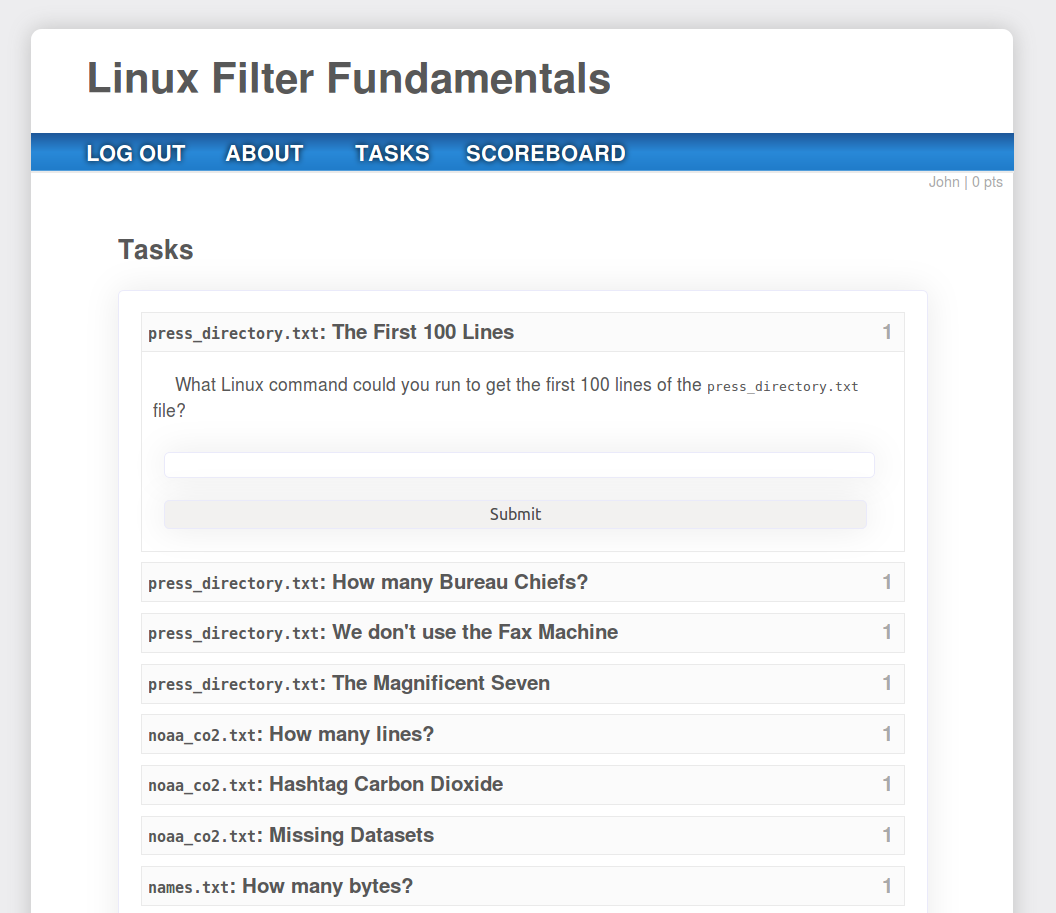
\includegraphics[width=500px, keepaspectratio]{filter_activity.png}}
		\centering
	\end{center}

	\hrulefill

	\newpage

	\subsubsection{The JSON Challenges}

	\begin{lstlisting}[language=bash]
"challenges": [

	{ 
		"title": "<code>press_directory.txt</code>: The First 100 Lines",

		"prompt": "
		<p> 
		What Linux command could you run to get the first 100 lines of the <code>press_directory.txt</code> file? 
		</p>
		",

		"possible_answers": [ 
			"head -n 100 press_directory.txt",
			"head -n100 press_directory.txt",
			"cat press_directory.txt | head -n 100",
			"cat press_directory.txt | head -n100",
			"cat press_directory.txt |head -n100",
			"cat press_directory.txt |head -n 100",
			"cat press_directory.txt|head -n 100",
			"cat press_directory.txt|head -n100"
		],
		
		"downloadable_files": [],
		"points" : 1
	},
\end{lstlisting}	

	\paragraph{} As I said, the only difference between this activity and the Scavenger Hunt is the JSON configuration file, with a new set of challenges. 

	\paragraph{} I won't show all the challenges above, but as you can see it is the same kind of style and syntax as the previous JSON config file.

	\paragraph{} \textbf{Note that for challenges that ask for a specific kind of command, you have to account for \textit{all} kinds of solutions}. That means accounting for whitespace, the order of commands, syntax style, etc..

	\paragraph{} Admittedly, that \textit{sucks}. And it trips up some students if \textit{their} solution isn't in \textit{your} listing. 

	\paragraph{} Currently I don't know any valid (or easy) solutions to this. I suppose it could be possible to test if their command gets the same output as what your solution does; but that requires running their code in a testbed which could be insecure.... Or perhaps you could remove the ``what kind of command'' questions entirely.

	\paragraph{} At this point, \textit{you} are the developer, and the choice is yours.

	\newpage

	\section{SSH Activity}

	\paragraph{} This was the first time that I as a teacher took the students away from Training Wheels. Rather than giving them instructions one-by-one, bite-size in the procedural Training Wheels environment, this time I just gave them a whole document to read.

	\paragraph{} I think of this as treating that class individual class period similar to a ``lab,'' like for other classes in the Electrical Engineering section at USCGA. The SSH Activity was the first activity after finishing Lesson \#10 of Training Wheels, ``Adding and Removing Users.'' 

	\paragraph{} Typically in lab you are given a hefty hand-out or packet full of your instructions; then it is up to you as the student to follow through with the tasking.

	\paragraph{} With the SSH Activity, this is exactly what I did: I gave the students a huge block of text and then just trusted them to read it, and follow along with the instructions.

	\paragraph{} Normally, I don't like this style of teaching --- because I hesitate to call it \textit{teaching} --- typically when you are given a wall of text to read your eyes tend to glaze over. I have been humbled, however: many students told me that they enjoyed it because they were able to follow along in their terminal and still poke and play as they used to.

	\paragraph{}

	\begin{center}
		\graphicspath{ {.} }
		\makebox[\textwidth]{
\includegraphics[width=150px, keepaspectratio]{mark.png}}
		\centering
	\end{center}

	\paragraph{}

	\paragraph{} This guide and all of the others that I have created for the class are written in Markdown. I do this for rapid development, and because github renders Markdown beautifully. 

	\paragraph{} So, to have students read the article, I directed them to the \texttt{resources/networking.md} file on the class repository.

	\begin{center}
		\graphicspath{ {.} }
		\makebox[\textwidth]{
\includegraphics[width=230px, keepaspectratio]{github.jpg}}
		\centering
	\end{center}

	\paragraph{} This class is what introduced the students to \textbf{the fork bomb}, which they loved and what they turned into a running gag. Many students have told the on more than one occasion that \textit{this} was their favorite class, because they got to fork bomb everyone.

	\subsection{The Markdown Source}

	\begin{lstlisting}
October 18th, 2016
======================

> John Hammond | Intro to Linux 2016

--------------------------------------

Recap:
-----

Welcome back to __Intro to Linux!__

Last week, you learned in [Training Wheels] how to interact with the _root_ user and even create and manage user accounts on your own. 

If you don't remember, does the command `sudo` ring a bell? It is "Super User Do"! ... in that you can temporarily _borrow_ the _root_ users powers to escalate your privileges and do things like install new software, add new users, or manage essential parts of the file system.

For Today's Class...
-------

Today, we'll be brushing the dust off of the `sudo` command and just briefly reviewing how to add a user. Then, we'll explore some simple networking things that [Linux] can do for us, an awesome thing called [`SSH`][SSH], and some file permissions. 

Let's dive right in!
-------

	\end{lstlisting}	

	\paragraph{} I won't go into the detail of all of the Markdown here (because it is really just English), but I'm sure you can see the syntax is very easy to pick up.

	\paragraph{} If you haven't seen or heard of Markdown before, you should check it out and add it to your toolkit. It makes whipping out documentation very easy... and actually very \textit{fun.}

	\paragraph{} Seeing how quickly and how simply you can make things beautiful is always awesome.

	\newpage

	\subsection{The Learning Content}

	\paragraph{} The guide and activity walks the students through creating a new user, which they \textit{intend} to let their friend use to SSH into their box. Each students creates a new user account with an easy and simple and password that they willing give to the person beside them.

	\paragraph{} Following creating the user, they run \texttt{ifconfig} to determine their own IP address, and share that with their neighbor as well. The two individuals exchange addresses and credentials, so they can successfully SSH into each other's machine.

	\paragraph{} Once they are logged in, the article encourages them to look around, try and create files, and interact with the file system. It explains why they receive all these \texttt{Permission denied} errors and tries to show off the 7-bits for \textit{file permissions}. 

	\paragraph{} I even remind them of \texttt{sudo} access, and have them try to run commands as root. This obviously fails, and it gives me as the teacher a venue to discuss the \texttt{sudoers} file. 

	\paragraph{} Those actions are really the only thing I wanted to expose them to; but I try edge them on as to what other kinds of things can they do, even without \texttt{root} access. This is where I introduce them to a fork bomb.

	\begin{center}
		\graphicspath{ {.} }
		\makebox[\textwidth]{
\includegraphics[width=230px, keepaspectratio]{forkbomb.png}}
		\centering
	\end{center}

	\paragraph{} The next class on the agenda following the SSH Activity was to introduce them to \texttt{bash} scripting. To whet the student's appetites, I wrote a simple script that would try and log into to all of the machines on the network, with the default credentials that I suggested in the article. I showed them the script on the projector and television screens, had them explain to me what they thought it did (simply by reading the source), and then running it so they could watch.

	\paragraph{} My priority is to teach them that: with everything, manual interaction is a \textbf{must}, but automation is \textit{divine}.

	\begin{center}
		\graphicspath{ {.} }
		\makebox[\textwidth]{
\includegraphics[width=150px, keepaspectratio]{shebang.png}}
		\centering
	\end{center}


	\section{The Scripting Playground}

	\paragraph{} In my eyes, the Scripting Playground was a little ambitious for the 2016 Linux class. I think I gave the students all the tools and materials that they really needed to accomplish the task, but they didn't have enough time to really brainstorm and craft their solution.

	\paragraph{} All of the material for this exercise is (at the time of writing) in the \texttt{scripting/} directory in the class repository.

	\subsection{The Vision}

	\paragraph{} This lesson has another Markdown article, that I intended the students to read first. It explains concepts like the sha-bang line, how to run a script, how to make the script executable, and it covers various examples of syntax for different logic in \texttt{bash}. Initially, I encouraged the students to play around and make small scripts for themselves to try the syntax with.

	\paragraph{} For the actual activity... it had big goals.

	\paragraph{} The idea was that the was another web server running, a forked version of the CTF Platform (the Scavenger Hunt and the Filters Activity you have seen before), but this time one without ``Jeopardy-style'' challenges. 

	\paragraph{} The CTF Platform would read in flags that were submitted \textbf{\textit{by the command-line}}. This way, the students would be encouraged to \textit{script} and automate their solutions.

	\paragraph{} The real \textit{challenge} for the game was actually scraping through a large github repository, that was cooked have to random commit messages, random programs, with random outputs. The student's goal was to automate looping through all of the repsitory commit messages, and switching to each commit to run each program. Each program would output another flag that they could submit for more points. And best of all; the program would seed the flag based off of the current minute; so you could submit a new flag every minute, and get more points!

	\paragraph{} I'm sure you can see how I now consider this ``ambitious.'' 

	\subsection{The Backend Server}

	\paragraph{} I said that this was a ``fork'' of the original CTF platform that you saw with the Scavenger Hunt and the Filters Activity. It just had a few modifications to handle the rotating flags.

	\begin{center}
		\graphicspath{ {.} }
		\makebox[\textwidth]{
\includegraphics[width=130px, keepaspectratio]{flag.png}}
		\centering
	\end{center}

	\newpage

	\subsubsection{Python Server Modifications}

	\begin{lstlisting}[language=Python]
correct_answers = {}

def flag_rotator( services ):
	global correct_answers, previous_minute
	current_second = int(strftime("%S"))
	correct_answers = static_flags

	for program in program_names:
		flag_base = program + strftime('%I:%M%p')
		sha_hasher = sha1()
		sha_hasher.update(flag_base)
		flag = sha_hasher.hexdigest()

		correct_answers[ flag ] = 10 # the flag is worth 10 points

	if ( current_second != 0 ):
		seconds_to_wait = 60 - current_second
		warning("waiting ", seconds_to_wait)
		sleep(seconds_to_wait)
		warning("done waiting")

	round = 0
	while 1:

		success("FLAG ROUND", round, "="*50)
		correct_answers = static_flags

		for program in program_names:
			flag_base = program + strftime('%I:%M%p')
			sha_hasher = sha1()
			sha_hasher.update(flag_base)
			flag = sha_hasher.hexdigest()
			correct_answers[ flag ] = 10 # the flag is worth 10 points

		round += 1
		sleep( 60 )

# ...

flag_rotation = Thread( target = flag_rotator, args = ( configuration['services'],) )
flag_rotation.daemon = True
flag_rotation.start()
	\end{lstlisting}

	\hrulefill

	\paragraph{} Admittedly I dislike this code because I duplicate some procedure here; but I can't particularly avoid it without some patchwork global variables... which I also don't want to do. 

	\paragraph{} Also note that I hardcode a lot of values here, like the $60$ second flag rotation and the static $10$ points for some flags. Again, this puts a bad taste in my mouth -- but it is my own code. I could fix this; (so could you;) but currently my priority is putting all of this documentation together.

	\paragraph{} I am sure you can see that the \texttt{flag\_rotater} function is threaded, and it is an infinite loop that just fires every minute. 

	\paragraph{} I use a SHA1 hash to ``generate'' the flag, and I just base it off of the name of the program along with the current minute. The \texttt{program\_names} list is actually defined outside of this function, and its value is just each line of a external file, which is a list of all the random programs that are generated by the \texttt{setup\_game.sh} script.

	\paragraph{}

	\begin{lstlisting}[language=Python]
commit_hashes_handle = open("commit_hashes.txt")
commit_hashes = commit_hashes_handle.read().split('\n')
static_flags = { commit_hash : 1 for commit_hash in commit_hashes }

program_names_handle = open("program_names.txt")
program_names = [ "./" + p for p in program_names_handle.read().split('\n') ];
	\end{lstlisting}

	\paragraph{} Remember, the flags that I put in play are the commit hashes of all of the github commit messages (the SHA1 identifiers) and the rotating flags from each binary. That means that the git commit IDs stay static; they don't change. The flags that come from the \texttt{program\_names} \textit{do change} every minute, with the above \texttt{flag\_rotator} function.

	\paragraph{} All of the above code is what allows the functionality for the rotating flags. Along with this, we need the functionality for the users to submit flags from the command-line. I accomplish this by essentially cloning the \texttt{check\_answer} function. (Again, duplicate code. If you're finicky, you can fix this.)

	\begin{center}
		\graphicspath{ {.} }
		\makebox[\textwidth]{
\includegraphics[width=120px, keepaspectratio]{sublime_text.png}}
		\centering
	\end{center}

	\newpage

	\begin{lstlisting}[language=Python]
@app.route("/submit", methods=[ "POST" ])
def submit(): 

	global correct_answers

	if request.method == "POST":
		if ( request.form['flag'] in correct_answers.keys() ):

			flag = request.form['flag']

			cur = g.db.execute('select score, solved_challenges from users where uuid = (?)',
				[ request.form['uuid'], ])

			current_score, solved_challenges = cur.fetchone()
			solved_challenges = solved_challenges.split()

			if ( flag in solved_challenges ):
				return 'You already submitted this flag!\n'

			new_score = current_score + correct_answers[flag]
			solved_challenges.append( flag + " " )
			cur = g.db.execute("update users set score = (?), last_submission = (SELECT strftime('%s')), solved_challenges = (?) where uuid = (?)", [
					new_score, 
					' '.join(solved_challenges),
					request.form['uuid']
				] );

			session['score'] = new_score
			g.db.commit();
			return 'Correct!\n';
		else:
			return 'Incorrect!\n';
	\end{lstlisting}

	\paragraph{} This function essentially makes for a more ``user-friendly'' function to work with for command-line submission, which I expect to be done with \texttt{curl}. 

	\paragraph{} I explain the usage of this function on the front-end of the website. All you need to do is \texttt{POST} to this URL with your own unique identifier (your account's \texttt{uuid}, which is given to you) and the flag that you are submitting. This will respond with a human-readable ``Correct'' or ``Incorrect'', rather than obscure JSON response, like we had earlier in the \texttt{check\_answer} function.

	\newpage


	\paragraph{} With this use of a \texttt{uuid}, we have to add this in the database and in the account creation.

	\paragraph{} This changes the registration function code to instead use this:


	\begin{lstlisting}[language=Python]
	# I use this for command-line submission...
	identifier = str(uuid4())

	cur = g.db.execute('insert into users (username, password, solved_challenges, score, last_submission, uuid) values ( ?, ?, ?, ?, ?, ? )', [ 
               request.form['username'], 
               sha256_crypt.encrypt( request.form['password']),
               "",  # No challenges completed
               0,   # no score.
               0,   # no last submission time,
               identifier # and a completely unique idenitifier
		  ] )

	g.db.commit()
	\end{lstlisting}

	\paragraph{} And...

	\subsection{The New Database Schema}

	\begin{lstlisting}[language=SQL]
drop table if exists users;
create table users (
  id integer primary key autoincrement,
  username text not null,
  password text not null,
  solved_challenges text not null,
  score integer not null,
  last_submission integer not null,
  uuid text not null
);
	\end{lstlisting}

	\paragraph{}

	\begin{center}
		\graphicspath{ {.} }
		\makebox[\textwidth]{
\includegraphics[width=270px, keepaspectratio]{sqlite.png}}
		\centering
	\end{center}

	\newpage

	\subsection{The Game Setup Script}

	\paragraph{} Once again I use my typical \texttt{bash} script style to automate the setup of the game. This has a different script than setting up the server; this is specifically \texttt{setup\_game.sh}.

	\paragraph{} As usual the code is lengthy and will span across multiple pages; so please bear with me.


	\begin{lstlisting}[language=bash]
#!/bin/bash
# @Author: John Hammond
# @Date:   2016-10-22 10:59:45

# Optional variables: modified by the cmd-line arguments
USERNAME=""

REPO_NAME="scripting_playground"
PROGRAM_NAMES="program_names.txt"
COMMIT_HASHES="commit_hashes.txt"

RED=`tput setaf 1`							# code for red console text
GREEN=`tput setaf 2`						# code for green text
NC=`tput sgr0`									# Reset the text color

function display_help() {
	cat <<EOF
usage:
	$0 -u USERNAME
parameters:
	-u
		Your username to log into Github.
	-h
		Display help message
EOF
}

function create_a_new_list_of_program_names(){
	echo "" > $PROGRAM_NAMES
}
	\end{lstlisting}

	\paragraph{} The only argument that the script takes is the github username, under which account it will create new \texttt{scripting\_playground} repository, which it will then fill with all of the random files.

	\paragraph{} To accomplish this, I utilize the Github API. \texttt{git} itself will prompt you for your password and it will not echo it onto the screen. In my case, I just used my personal ``JohnHammond'' github account.

	\paragraph{} Also, notice the general function I use to create a new list of program names. I use \texttt{echo} here with some redirection to overwrite anything that may already exist and start fresh.

	\newpage

	\subsubsection{Creating the Repository}

	\begin{lstlisting}[language=bash]
function create_new_repository(){

	while [ 1 ]
	do
		echo "$FUNCNAME:$GREEN creating repository $REPO_NAME $NC"
		response=`curl -u "$USERNAME" https://api.github.com/user/repos -d "{\"name\":\"$REPO_NAME\"}"`

		echo $response | grep "Bad credentials" > /dev/null 2>&1
		if  [ $? -eq 0 ]
		then
			echo "$FUNCNAME:$RED bad password for $USERNAME! $NC"
			continue
		fi
		echo $response | grep "already exists" > /dev/null 2>&1
		if  [ $? -eq 0 ]
		then
			echo "$FUNCNAME:$RED The repository already exists! $NC"
			exit -1
		fi
		break
	done

}

function clone_the_new_repository(){

	git clone "https://github.com/$USERNAME/$REPO_NAME"
	cd $REPO_NAME
}


function copy_readme_to_the_new_repository(){

	cp ../game_readme.md README.md
	git add .
	git commit -m "Added original README.md"
}
	\end{lstlisting}

	\paragraph{} As I said before, I use the Github API to handle the work with creating the new github repository. \textbf{Note that a repository with the same name cannot already exist; if this is the case, the script will fail, and you must remove that repository on your own.}

	\paragraph{} Then, I just generalize another new function to clone the repository and move into it. I do this again with moving in the \texttt{README.md}.

	\newpage

	\subsubsection{Adding the Binaries to the Repo}

	\begin{lstlisting}[language=bash]
function commit_new_program(){

	program_name=`head /dev/urandom | md5sum | cut -d " " -f1 | base64`

	echo "$FUNCNAME:$GREEN commiting program $program_name $NC"

	# I get rid of the case so the program name and commit message are not equivalent
	# This way a person could not reverse engineer the flags by just the commit message alone
	commit_label=`echo $program_name | tr [:upper:] [:lower:]`

	cp ../minutehash $program_name
	git add . 
	git commit -m "$commit_label"

	echo -e "$program_name" >> ../$PROGRAM_NAMES

	rm $program_name
}

function get_commit_hashes(){

	git rev-list --all --remotes > ../$COMMIT_HASHES
}
	\end{lstlisting}	

	\paragraph{} The \texttt{setup\_game.sh} script is the one that creates all the random binaries in the repositories. The whole generation process is automated, so you can spin up as many random programs as you would like.

	\paragraph{} You should be able to see that the core program that I am using to duplicate here is the \texttt{minutehash} program. I will go over the source of that very soon; but is essentially just a C++ binary that spits out the SHA1 hash of its own name and current minute (the flag)!

	\paragraph{} It adds and commits each program, and adds it to the list that we are using to keep track of all the program names. Since that is really the ``seed'' for the flag, both the repository \textit{and the backend server} need to know the names. 

	\paragraph{} Then, I remove the local copy of the binary.

	\paragraph{} Also above, I showcase the syntax that I use to gather all of the commit message ID numbers (the static flags).

	\newpage


		\subsubsection{General Functions}

	\begin{lstlisting}[language=bash]
function push_changes(){

	git push
	cd ..
}

function remove_the_local_repository(){

	rm -rf $REPO_NAME
}

# Parse script options
while getopts u:h opt; do
	case $opt in
		u)
			echo "$0: ${GREEN}using github username ${OPTARG}${NC}"
			USERNAME=$OPTARG
			;;
		h)
			display_help
			exit 0
			;;
		\?)
			exit -1
			;;
	esac
done

# Make sure we entered a database name
if [ "$USERNAME" == "" ]; then
	echo "$0: ${RED}you must specify your github username!${NC}"
	display_help
	exit -1
fi
	\end{lstlisting}	

	\paragraph{}

	\paragraph{} Above are some ``house-keeping'' functions, and the initial tests before the main function call to make sure you as the developer are invoking the script correctly.

	\paragraph{} Finally, after all the functions are built, we can invoke the main function, which should at this point read like a story book.

	\paragraph{}

	\hrulefill

	\newpage

	\subsubsection{The Main Function}

	\begin{lstlisting}[language=bash]
function main(){

	create_a_new_list_of_program_names

	create_new_repository
	clone_the_new_repository
	copy_readme_to_the_new_repository

	for i in {1..300}
	do
		commit_new_program
	done

	get_commit_hashes

	push_changes

	remove_the_local_repository

}
	\end{lstlisting}	

	\paragraph{} And that is all that is needed to set up the game. You can create as many of the random programs as you would like; the more that exists, the more that the users have to comb through... but since they would be ideally writing a script to solve the problem, the number would not matter.  

	\paragraph{} After running the script, the two files that act as the bridge between the game and the server, \texttt{program\_names.txt} and \texttt{commit\_hashes.txt} should be populated with random names and hashes:

	\paragraph{} Sample \texttt{program\_names.txt}:

	\begin{lstlisting}[language=bash]
M2NhZTNiODM2ZjdiYzdjMTViNzk4ZDA2N2EwZTI3OWUK
ZTI5ZTQzMDg4ZGU5MzU2MTg5N2M1YjJkY2Q5NGZhOGIK
ODIwOTdiNGNiNzlkOWNlODM3OTE0MWRjZWUwZTYzYzQK
MmUxMjgzMDMyMzJmNDliN2QxYWQzOGU3ODUzY2I4ZmUK
...
\end{lstlisting}	

\paragraph{} Sample \texttt{commit\_hashes.txt}:

	\begin{lstlisting}[language=bash]
3f43a88cc832c0cdecc98f4bb389ec0309d94b16
4c047698e05a9c5c2663ff547b6019086dd218bf
706408355a9d21ad568bdd60e0c3163511a04108
ffd5db09a38afeaf119430b9148c8eb44d6941a9
1af96f8f4c92aceebb2861216cbbe87cceece4dd
...
\end{lstlisting}

	\newpage

	\subsection{The Random Binary ``Minutehash''}

	\paragraph{} The random binary that lives in each git commit in the repository has only one purpose: to spit out a flag, which is seeded by the name of the program (random) and the current minute (so the flags rotate over time).

	\paragraph{} This is a simple thing in C++. I use Steve Reid's SHA1 code, which I found online and is ``100\% in the public domain.'' I won't showcase his hashing source code, but I'll showcase how I use it in my \texttt{minutehash.cpp}.\\



		\begin{lstlisting}[language=c++]
/*
* @Author: John Hammond
* @Date:   2016-10-20 08:38:34
* @Last Modified by:   John Hammond
* @Last Modified time: 2016-10-20 14:40:04
*/

#include <iostream>
#include <time.h>
#include <string.h>
#include "sha1.h"
#define SIZE_OF_BUFFER 8

using namespace std;

int main( int argc, char *argv[] ){

	time_t raw_time;
	struct tm * timeinfo;
	char buffer[SIZE_OF_BUFFER];

	time( &raw_time );
	timeinfo = localtime(&raw_time);

	// This gets the current minute as a string... (like 02:34PM)
	strftime(buffer, SIZE_OF_BUFFER, "%I:%M%p", timeinfo );

	// This adds on to the filename the current minute...
	strcat(argv[0], buffer);

	cout << sha1(argv[0]) << endl;

	return 0;
}
\end{lstlisting}

	\newpage

	\paragraph{} I whipped out a super simple \texttt{Makefile} for this, to make everyone elses' lives easier if they ever inherit all of this.

	\begin{lstlisting}[language=make]
all:
	g++ minutehash.cpp sha1.cpp -o minutehash

clean:
	rm minutehash
\end{lstlisting}

	\paragraph{} And I move the compiled \texttt{minutehash} executable into the \texttt{scripting/} directory itself, so the \texttt{setup\_game.sh} script can reach it easily.

	\subsubsection{Beware of Architecture}

	\paragraph{} At this point, I warn you to think of your end-user platform. If the students are on the Raspberry Pi, your \texttt{minutehash} binary must also be compiled for the Raspberry Pi architecture.

	\paragraph{} I mentioned this briefly in the introduction; but this had bit me during a class. As a content creator and developer, I compiled \texttt{minutehash} on my Intel processor. 

	\paragraph{} The Raspberry Pi uses ARM. 

	\paragraph{} \textbf{Here be dragons}.

	\subsection{The Backend Server Setup Script}

	\paragraph{} The setup script for the Python and Flask web server, \texttt{setup.sh}, is the essentially same as it was for the original CTF Platform (Scavenger Hunt/Filters Activity). The only addition is that it now invokes the \texttt{setup\_game.sh} script, and takes in a github username as an argument (to pass it to the \texttt{setup\_game.sh} script).

	\paragraph{} This is so you as the developer only have to run \textit{one} script to spin up the whole exercise. 

	\paragraph{} I won't show the code for the new additions; all it is is the new \texttt{USERNAME} variable, tested as an argument on startup, and then a line in the \texttt{main} function to call the \texttt{setup\_game.sh} script with the \texttt{USERNAME} variable. \\


	\begin{center}
		\graphicspath{ {.} }
		\makebox[\textwidth]{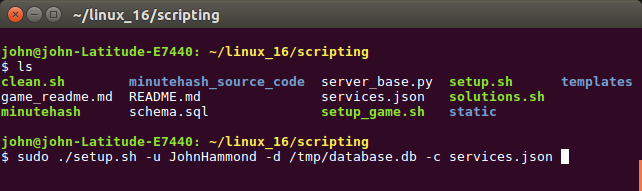
\includegraphics[width=480px, keepaspectratio]{setup_scripting.png}}
		\centering
	\end{center}

	\newpage

	\subsection{The JSON Configuration}

	\begin{lstlisting}[language=C++]
{
	"app_title" : "Scripting Playground",

	// ... navigation not included for this excerpt...

	"app_about": "
		<p>
		The idea behind this Scripting Playground is to use <code>git</code> as a vessel to teach <code>bash</code> scripting. In some commits, there is an executable file, that once run, will yield a flag based off of the current time. The goal is to write a script that will run through each commit, run each program, and submit each flag -- each minute.
		</p>
		<p>
		This could be done by hand of course, but it would be tedious and not very fruitful in regard to the game. So, the more you can script, the more you win!
		</p>
		<h2>Good luck and have fun!</h2>
	",

	"services": [
		{ 
			"title": "<a href='https://github.com/JohnHammond/scripting_playground'>A New github Repository</a>",
			"description": "
				This repository contains an executable that will give you a flag. 
				In each commit there is another executable, and even the commit SHA1 hashes themselves
				are flags you can submit for points.
			",
			"points" : 10
		}
	]
}
\end{lstlisting}

	\paragraph{} The \texttt{services.json} configuration file does not have any challenges, like the other \texttt{.json} files in the usual CTF platform. This time it just notes \texttt{services}, with a link explaining the github repository.

	\paragraph{} Note that \textbf{my repository} is currently hardcoded in. I have not yet made a way for the \textbf{setup.sh} script to talk with this configuration file. If you use a different repository (which you will have to, because you are not me), you will have to change this on your own.

	\newpage

	\subsection{The Solutions}

	\paragraph{} My solution may not be the most efficient, and it may not be what everyone else comes up with; but it seems to get the job done.

	\paragraph{} Below are some general functions that I use. First, to clone the repository and move into it, and another wrapper to submit a flag, so I don't have to type out that \texttt{curl} syntax over and over.

\begin{lstlisting}[language=Bash]
#!/bin/bash

function clone_repo(){
	git clone "https://github.com/JohnHammond/scripting_playground"
	cd scripting_playground
}

function submit_flag(){

	# THE CURL COMMAND FOR THIS WILL VARY
	# SINCE THE uuid OF THE USER WILL BE GENERATED
	# BY THE SERVER
	curl -k "http://localhost:444/submit" --data "uuid=9644903a-bab2-4eb9-b0b3-d83c7a65c305&flag=$1"
}
\end{lstlisting}

	\paragraph{} Obviously the URL and the \texttt{uuid} variable will have be changed for your environment and user account.

	\paragraph{} The next function is what grabs all of the commit hashes and submits them. \\

	\begin{lstlisting}[language=Bash]
function submit_commit_hashes(){
	git rev-list --remotes | while read line
	do
		submit_flag $line
	done
}
\end{lstlisting}

	\paragraph{} I use the same exact syntax as before to grab all the commit hashes. This time, I just loop through them line by line, and submit them with my wrapper function. \\

	\begin{center}
		\graphicspath{ {.} }
		\makebox[\textwidth]{
\includegraphics[width=200px, keepaspectratio]{curl.jpg}}
		\centering
	\end{center}

	\newpage

	\paragraph{} The next function is what loops through all of the commits, checks out each commit, runs the program, and submits its output.

	\begin{lstlisting}[language=Bash]
function submit_all_programs(){

	git rev-list --remotes | while read line
	do
		git checkout $line > /dev/null 2>&1
		program_name=`ls | grep -v README.md`
		./$program_name

	done | while read line
	do
		submit_flag "$line"
	done
}
\end{lstlisting}

	\paragraph{} Notice that I \texttt{grep} out the \texttt{README.md} file, because that is the only other file in the repo that will not execute and give me a flag. 

	\paragraph{} This all done in the script, and then I clean up by removing the directory. 

	\paragraph{} If you wanted to, though, you could just slap the above function in a \texttt{while} loop to run every sixty seconds and keep getting you points off of the rotating flags.

		\begin{lstlisting}[language=Bash]
clone_repo

submit_commit_hashes
submit_all_programs


cd ..
rm -rf scripting_playground

# And you could then loop the submission to get flags every minute..
# while [ 1 ];
# do
# 	sleep 60
#  done
\end{lstlisting}

	\paragraph{} \paragraph{} \paragraph{}

	\hrulefill

	\newpage

	\subsection{Use at Your Discretion}

	\paragraph{} I don't think I have to reiterate that not all of this is good code.

	\paragraph{} I also don't think I have to reiterate that this is may be too ``ambitious'' for students who are just starting to learn Linux.

	\paragraph{} I would like to think that this is just me trying to encourage students to learn and try more difficult and challengings things, but it could very well just be me dragging through the fire.

	\paragraph{} Admittedly, there is no easy way to \textit{teach} scripting.

	\paragraph{} Well, sure, you can teach someone syntax, but teaching the \textit{innovation} is much harder to do. That has been my goal with the Scavenger Hunt and other ``game'' like activities; and I would say that this was my same intent with the Scripting Playground. 

	\paragraph{} However, for a one-credit course, that met once a week for one hour... I couldn't spend as much time as what might have been necessary to really get everything out of this exercise.

	\paragraph{} Regardless if this class becomes a much larger course, with more time involved, perhaps this could be a good activity. When I look at my solutions, I don't think it is too difficult...

	\paragraph{} ... but I am no longer the judge: \textbf{you are.}

	\paragraph{} \paragraph{}\paragraph{} \paragraph{}

	\begin{center}
		\graphicspath{ {.} }
		\makebox[\textwidth]{
\includegraphics[width=400px, keepaspectratio]{hats.jpg}}
		\centering
	\end{center}

	\paragraph{} \paragraph{} \paragraph{} \paragraph{}

	\hrulefill

	\newpage

	\section{Installing Software Guide}

	\paragraph{} The Installing Software Guide was another Markdown document that I gave to the students and had them walk through it on their own.

	\paragraph{} At the time of writing, the article is in the online repository under the \texttt{installing\_programs} directory.

	\subsection{The Learning Content}	

	\paragraph{} This document was much larger than the last; I was hopeful the students would be able to endure more reading. The material covered goes into:

	\begin{itemize}
		\item Compiling Source Code
		\begin{itemize}
			\item Writing C
			\item Using \texttt{gcc} for basic Compilation
		\end{itemize}
		\item Building a Makefile
		\item Working with Tarballs
		\begin{itemize}
			\item Creating a Tarball
			\item Extracting a Tarball
		\end{itemize}
		\item Installing Software from the Package Repositories
		\begin{itemize}
			\item Updating the Repositories
			\item Searching for a Package
			\item Installing a Package
		\end{itemize}
	\end{itemize}

	\paragraph{} I walk the students through using \texttt{nano} as their simple command-line text editor. I explain to them what preprocessor definitions are in C, and how to compile and run their software. This is likely the first time the students have seen \texttt{gcc}, since many have been handicapped by Microsoft Visual Studio.

	\begin{center}
		\graphicspath{ {.} }
		\makebox[\textwidth]{
\includegraphics[width=150px, keepaspectratio]{C.png}}
		\centering
	\end{center}	

	\hrulefill

	\newpage

	\paragraph{} I also try and expose them to what \textbf{tarball} is, how to create one, and extract one. 


	\begin{center}
		\graphicspath{ {.} }
		\makebox[\textwidth]{
\includegraphics[width=100px, keepaspectratio]{tarball.png}}
		\centering
	\end{center}	


	\paragraph{} As a real-world example to work with, I have them extract and \texttt{make} the \texttt{figlet} software package. 

	\begin{center}
		\graphicspath{ {.} }
		\makebox[\textwidth]{
\includegraphics[width=300px, keepaspectratio]{figlet.png}}
		\centering
	\end{center}	

	\paragraph{} Following this I do explain to them that it is not common to install software by compiling the source code; but it is advised to know \textit{how}.

	\paragraph{} For the 2016 Intro to Linux class, we had this class after students took part in a ``distribution project,'' where they were to research and write about a Linux distribution. In many cases, they explained what kind of \textit{package manager} the distribution used. This was a good tie-in, because we could showcase Aptitude on the Rasbian distro.

	\paragraph{} As an example, I had to students install \texttt{cowsay} with the command-line package manager.

	\paragraph{}

	\begin{center}
		\graphicspath{ {.} }
		\makebox[\textwidth]{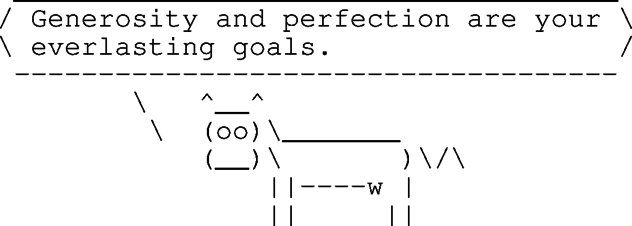
\includegraphics[width=300px, keepaspectratio]{cowsay.png}}
		\centering
	\end{center}	


	\paragraph{} This lesson did not include too much technical content on the side of the content creator. I believe that that is an okay thing (I can't think of any good ways to make an activity out of installing and compiling software packages)... but if you as the future instructor want to expand on it, you have the blessing of many ASCII cows.

	\paragraph{} \paragraph{}

	\hrulefill

	\newpage

	\section{The Web Exploit Exercise}

	\paragraph{} The Web Exploit Exercise was meant to be a morale exercise. For the 2016 Intro to Linux class, this was the Tuesday just before Thanksgiving break, so I wanted to give the students a little bit more fun and interesting to explore. 

	\paragraph{} The execution of the exercise faced some stumbling blocks, but I still think it was a successful activity.

	\subsection{The Idea}

	\paragraph{} The idea behind the Web Exploit Exercise was that instead of me as the instructor usually giving them a large document full of instructions, or by guiding them with some training materials or leading questions, this time they would be given a puzzle.

	\paragraph{} I intended to write on the board a simple IP address. And that was all the information I planned on giving them; I thought I would give them no explanation; maybe an address and perhaps one goal: ``get root access.''

	\paragraph{} My hope was that they would struggle a little bit, but start to do some critical thinking and explore on their own.

	\subsection{The Website}

	\paragraph{} The IP address that I would give the students was a website.

	\paragraph{} I cooked up a fake and simple website, spoofing a company with the name given as ``Allsafe.'' \textbf{This entire exercise was meant to be an homage to the hacking community's favorite TV show, the recent USA hit: Mr. Robot}.

	\paragraph{}

	\begin{center}
		\graphicspath{ {.} }
		\makebox[\textwidth]{
\includegraphics[width=350px, keepaspectratio]{mr_robot.png}}
		\centering
	\end{center}	

	\paragraph{}	

	\paragraph{} The website was intentionally very simple. The students were to do some reading and reconnaissance on the website to see what kind of software it was using, and to uncover the employees that worked there.

	\paragraph{} I scraped the design off of some free online template. It's full of bloated HTML and CSS, so I won't care to showcase the source code here.

	\newpage

	\begin{center}
		\graphicspath{ {.} }
		\makebox[\textwidth]{
\includegraphics[width=470px, keepaspectratio]{allsafe.png}}
		\centering
	\end{center}	


	\paragraph{} I hoped the student would move around between all of the links, noting especially the ``Products.'' This page gives them some more insight as to what they should do. \\

		\begin{center}
		\graphicspath{ {.} }
		\makebox[\textwidth]{
\includegraphics[width=470px, keepaspectratio]{products.png}}
		\centering
	\end{center}	

	\newpage

	\paragraph{} The tip here is that the web server also has an SSH server, and their employee credentials are explained right on the webpage.

	\paragraph{} I write that the username is the employee's first name, and their password is their lastname and their employee number. 

	\paragraph{} \textbf{What I fail to mention is that these are all lowercase.} This was a real stumbling block for students; I should have been more specific in the username and password, explaining that I used \textit{all lowercase} for the credentials. \textbf{Be cautious of that if you use this exercise.}

	\paragraph{} If you check out the employees that work at Allsafe, you will see only three: Elliot, Angela, and Gideon. These three act as the ``levels'' to the game. You progress from one to the next. If you explore the pages, you should see that only Elliot has his employee number visible. \\

	\begin{center}
		\graphicspath{ {.} }
		\makebox[\textwidth]{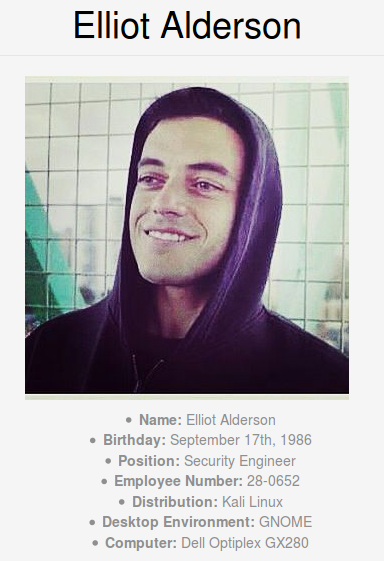
\includegraphics[keepaspectratio]{elliot.png}}
		\centering
	\end{center}		

	\newpage

	\subsection{Elliot}

	\paragraph{} With the found information, ideally the student would try and login to the server with SSH.

	\begin{lstlisting}[language=Bash]
# entering password: alderson28-0652

ssh elliot@10.6.1.155
\end{lstlisting}

	\paragraph{} Obviously the IP address will differ if you set up this game on your own.

	\paragraph{} Once you log in as Elliot and explore, you should see a hefty amount of text files in his home directory.

		\begin{center}
		\graphicspath{ {.} }
		\makebox[\textwidth]{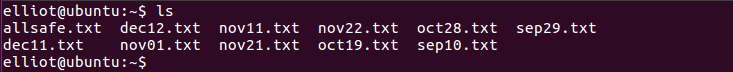
\includegraphics[width=400px, keepaspectratio]{elliot_home_directory.png}}
		\centering
	\end{center}		

	\paragraph{} Admittedly, almost all of these are red herrings. Each of them have cryptic and strange quotes from the Mr. Robot television show. The only one with real insight is \texttt{nov22.txt}, which was the date of the class that day. \\

	\begin{lstlisting}[]
We started using GPG at Allsafe, so I wanted to take some notes on how to use it. There is documentation online, but the best place to look is always in the man pages.

I left a file in the /usr/bin directory. It's the only one with a ".txt" extension.
\end{lstlisting}

	\paragraph{} This was meant to be a hint to refer to the \texttt{man} pages on \texttt{gpg}. All of this exercises was meant to be a fun review, while at the same time, mixing in some new technologies that the students may not have ever seen before. 

	\paragraph{} The other note in this file explains about a \texttt{.txt} file in the \texttt{/usr/bin} directory. Again, this is meant to be review; the students will have to check out the \texttt{/usr/bin} directory and \texttt{grep} for the necessary file. \\

		\begin{center}
		\graphicspath{ {.} }
		\makebox[\textwidth]{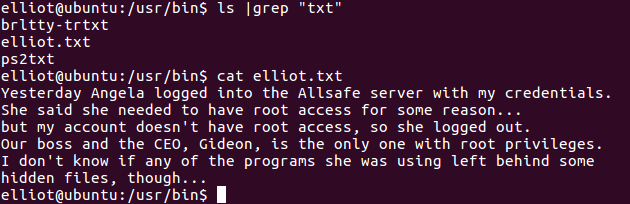
\includegraphics[width=400px, keepaspectratio]{elliot_note.png}}
		\centering
	\end{center}		

	\newpage

	\paragraph{} Hopefully the user reads this well enough to understand that their goal is to get access to Gideon's account. Since his is the CEO, he has root access on the box.

	\paragraph{} This is another hint to check out hidden files back in Elliot's home directory. If she had used his computer, there may be some \textit{history} left?

	\paragraph{} You should be able to \texttt{ls -a} and find some hidden files.

	\paragraph{} The user has to be very observant, here. There are two interesting files that should catch their eye: \texttt{.angela.txt.gpg} and \texttt{.history}.

	\paragraph{} Trying to read the GPG file will not work, because the file is encrypted. Hopefully they will know that, if they had read the man page for the \texttt{gpg} command. Instead, they can look at the \texttt{.history} file:

	\begin{lstlisting}[]
ls
whoami
cd
id
man gpg
clear
cd /usr/bin
ls
ls | grep "txt"
cat elliot.txt
cd
ls -a
exit
ls
nano passwords.txt
rm passwords.txt
nano credentials_for_angela.txt
mv credentials_for_angela.txt /tmp/nov22/
curl http://10.6.1.155/robots.txt
\end{lstlisting}

	\paragraph{} Hopefully here the user sees something interesting:.

	\paragraph{} \textbf{They edit and move a file called \texttt{credentials\_for\_angela.txt} into \texttt{/tmp/nov22/}!}

	\paragraph{} If you check out the \texttt{/tmp/nov22/credentials\_for\_angela.txt} file first, you will see it gives you the GPG key for the \texttt{.angela.txt.gpg} file.

\begin{lstlisting}[]

 Angela's GPG key is:

 backtothefuture2

		\end{lstlisting}

	\newpage

	\subsection{Angela}

	\paragraph{} Now, the student can decrypt that GPG file. If they read the man page, they could easily determine the syntax.

	\begin{center}
		\graphicspath{ {.} }
		\makebox[\textwidth]{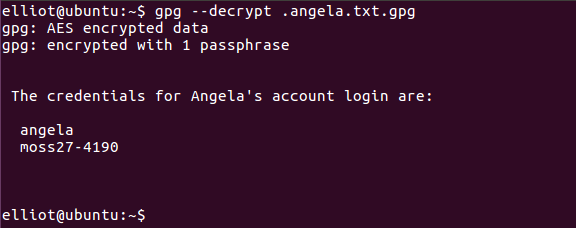
\includegraphics[width=400px, keepaspectratio]{angela_password.png}}
		\centering
	\end{center}		
	
	\paragraph{} And with that, they can log into the \texttt{angela} account. This is probably best done using \texttt{su}.

	\paragraph{} On the website, Angela's employee number is not visible. That's what you have to move through Elliot to get to the ``next level!''

	\begin{center}
		\graphicspath{ {.} }
		\makebox[\textwidth]{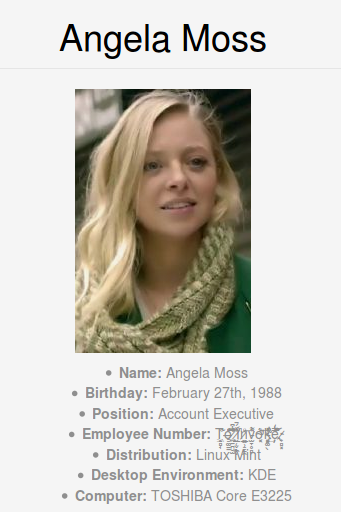
\includegraphics[width=230px, keepaspectratio]{angela.png}}
		\centering
	\end{center}
	
	\newpage

	\paragraph{} When you log in as Angela and you look around, you should be able to see a \texttt{Makefile} in the home directory. Again, this is review; hopefully the students knows how to interact with that \texttt{Makefile}!

	\begin{center}
		\graphicspath{ {.} }
		\makebox[\textwidth]{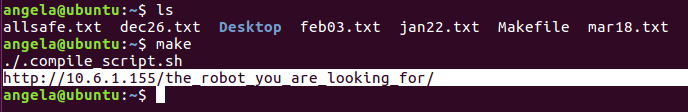
\includegraphics[width=400px, keepaspectratio]{angela_robot.png}}
		\centering
	\end{center}


	\paragraph{} You can see it pushes out a link. This link is back on the webserver... \\

	\begin{center}
		\graphicspath{ {.} }
		\makebox[\textwidth]{
\includegraphics[width=400px, keepaspectratio]{cron.png}}
		\centering
	\end{center}

	\paragraph{} Now this hints towards \texttt{cron}, something new for the students. I give them a link to documentation in case they want to read more about it, but I do explain that files are in the \texttt{/etc/cron.d/} directory.

	\paragraph{} In that directory there is an interesting file...

	\begin{center}
		\graphicspath{ {.} }
		\makebox[\textwidth]{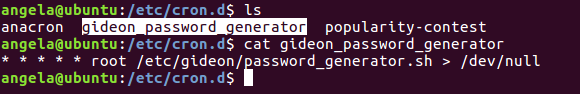
\includegraphics[width=400px, keepaspectratio]{gideon_password.png}}
		\centering
	\end{center}

	\paragraph{} This file is a typical \texttt{cron} task. It looks like it running a command as \texttt{root} every minute... and it is trying to run a file, \texttt{/etc/gideon/password\_generator.sh}. The student should be able to recognize this as a \texttt{bash} script, and they should take a look at it!


	\begin{center}
		\graphicspath{ {.} }
		\makebox[\textwidth]{
\includegraphics[width=300px, keepaspectratio]{allsafe_image.jpg}}
		\centering
	\end{center}

\newpage

\subsection{Gideon}

\begin{lstlisting}[language=bash]
#!/bin/bash

# Giden, our CEO, tries to keep his password super secure.
# So, he alternates his password, based on the MD5 hash of
# the current minute!

PASSWORD=`date +%M | md5sum | cut -d " " -f1`

echo "gideon:${PASSWORD}"| sudo chpasswd
\end{lstlisting}

	\hrulefill

	\paragraph{}

	\paragraph{} This \texttt{bash} code explains that Gideon's password is rotated every minute. It uses the \texttt{date} command to get the current minute (just the numebr 00 -- 59, as you can see with that format specifier) and that is hashed with an MD5 sum. 

	\paragraph{} The student could see this code and try and run it on their own. He could get the value of the \texttt{PASSWORD} variable, and log into the \texttt{gideon} account wth those credentials. They just have to be on the right side of the minute!

	\begin{center}
		\graphicspath{ {.} }
		\makebox[\textwidth]{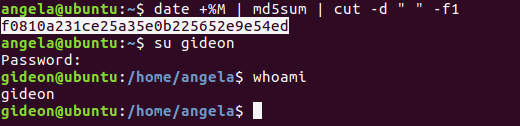
\includegraphics[width=300px, keepaspectratio]{got_gideon.png}}
		\centering
	\end{center}

	\begin{center}
		\graphicspath{ {.} }
		\makebox[\textwidth]{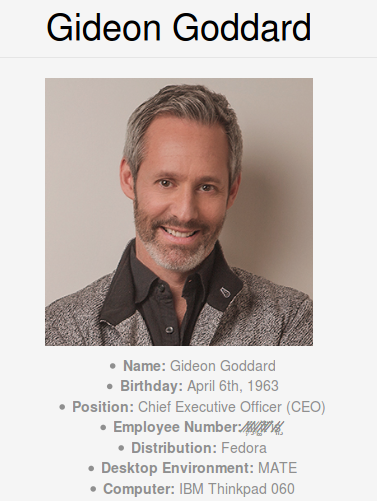
\includegraphics[width=200px, keepaspectratio]{gideon.png}}
		\centering
	\end{center}

	\newpage

	\subsection{Victory!}

	\paragraph{} With that, the student has ``won'' the game. The goal was just to get root access, and Gideon's account has \texttt{sudo privileges}.

	\paragraph{} I had to stress to that students that now that they had root access, the \textit{owned} the machine. The could do literally anything they wanted. What I encouraged some students to do was look more into the Apache webserver, and see if they could add a page for themselves on the website or tamper with the webpages.

	\subsubsection{Don't Trust all your Users}

	\paragraph{} For this small exercise, I spun up a virtual machine and just let all of the students SSH into it. I was hopeful that they would not ``vandalize'' -- like remove files that led to parts of the story or change user passwords -- but sure enough, they did.

	\paragraph{} I had to quickly recover some files as I saw them drop, and tell other students ``No, that's not the right password -- someone changed it -- hang on...'' and I am sure that took away from some of the experience. At least, it definitely did for me as the creator.

	\paragraph{} In an ideal environment we may be able to spin up a game for each individual student, like maybe some work with Vagrant or Docker, but the distribution of each of those personalized game environments might be another difficult problem to solve. 

	\subsection{Aftermath}

	\paragraph{} Regardless, I still think there was a lot of learning value in this exercise. Just over half of the dozen students in my 2016 class were able to successfully ``get Gideon.'' I believe if there wasn't the stumbling blocks of non-specific lowercase passwords and people vandalizing the files, everyone would have been able to win.

	\paragraph{} As I've said before, my hope with this exercise was to remove me from the equation and just let the students explore and try to break into this thing on their own. I wanted them to feel like they were doing their own penetration testing; going from a front-facing website to an SSH login shell. 

	\subsection{Reusability}

	\paragraph{} At the time of writing, not \textit{all} of the code and material to set up this exercises has been gathered and automated. 

	\paragraph{} In an ideal world I would have code to bootstrap a machine to host this activity, like I have for all of my other products, but for the design of this exercise it simply didn't happen.

	\paragraph{} However, because the game was hosted all in a virtual machine, I can offer the OVA file. At that point, management is up to you as the future content creator.	

	\paragraph{} Everything that is currently available is available on the online repository, in the \texttt{allsafe} directory.


	\newpage
	\section{MySQL Guide}
	
	\paragraph{} The MySQL Guide was the last class before exams. This time I again released a large Markdown document with instructions and a ``how-to'' style.

	\paragraph{} The document is available on the online repository in the \texttt{mysql} directory. 

	\paragraph{} For this class, I wanted to showcase and demonstrate use of MySQL from the command-line. Since many of the EEs taking the Intro to Linux class at USCGA will likely have capstone projects -- in Linux -- and will likely be using databases -- in Linux -- we figured they ought to know how to work with databases -- in Linux.

	\paragraph{} So, I wanted to show them the raw connection and communication with a MySQL database. The plan was to put them at the interpreter and let them enter SQL statements, so they could immediately see their action and the databases' response. I think working with an interactive shell is one of the best ways to learn, because you can explore and you have instant feedback.

	\paragraph{} They install the \texttt{mysql-server} package with Aptitude and just run the MySQL server on their own machine, and I give them the syntax to log in and create tables and all.

	\begin{center}
		\graphicspath{ {.} }
		\makebox[\textwidth]{
\includegraphics[width=300px, keepaspectratio]{mysql.png}}
		\centering
	\end{center}


	\paragraph{} This was the first time in class that I went through the entirety of the document \textit{with the students} and talked through it. In my opinion, it was probably the closest I had ever gotten to a ``lecture'' in the Linux class.

	\paragraph{} After we had gone through the article together, I showed them \texttt{sqlmap}. Now that they had seen how to create and put together a database and some syntax with the SQL language, I wanted them to see how SQL could be put to use in another, more offensive way.

	\paragraph{} Originally I tried to get them to install \texttt{sqlmap} by the repositories, but of course, the package wasn't in the Raspbian repos. Remember, this is another reason why I advise against the Raspberry Pi in a future class.

	\begin{center}
		\graphicspath{ {.} }
		\makebox[\textwidth]{
\includegraphics[width=300px, keepaspectratio]{sqlmap.png}}
		\centering
	\end{center}


	\paragraph{} I rolled with the punches and we went to download the source code from github. We were able to run it easily, and we all threw it against the Acuart Vulnerable Webpage.

	\paragraph{} That was able to leak out a fake e-mail account, name, phone number and credit card number. It was flashy enough to keep the students engaged and wow them with SQL. 

	\begin{center}
		\graphicspath{ {.} }
		\makebox[\textwidth]{
\includegraphics[width=400px, keepaspectratio]{acuart.png}}
		\centering
	\end{center}

	\paragraph{} Remember, this guide and the others are not much technical work; they are simply Markdown writeups, that you can easily modify if that is what you plan on using for a lesson.\\

	\begin{lstlisting}[]
Working with MySQL
================

You can interact with a SQL database in a much better and much more efficient way, compared to what you are probably used to when working with languages like C#, or trying to play-pretend with an Access database or Excel spreadsheet.

Installing MySQL Server and Client
----------

To install MySQL, please run

``` bash
sudo apt install mysql-server
```

\end{lstlisting}

\newpage

\section{The Distribution Project}

\paragraph{} The only ``project'' that was assigned during the 2016 Intro to Linux class was what was codenamed the ``Distribution'' project.

\paragraph{} I briefly mentioned it in a previous section, but the idea behind the project was that each student want randomly assigned a unique Linux distribution. They had a few weeks to research the distro, spin up a VM and play with it, and write a small essay (no longer than a page) on what they thought of this distro.

\paragraph{} This coudl range from why people use it, what purpose is it supposed to have, does it succeed, do you like it, why or why not, etc...

\subsection{The 2016 Distros}

\paragraph{} The distributions we used for this year were as follows:

\begin{itemize}
	\item Ubuntu
	\item CentOS
	\item Arch Linux
	\item Zorin
	\item Tails
	\item FreeBSD
	\item ElementaryOS
	\item Slackware
	\item Sugar
	\item Kali Linux
	\item OpenSUSE
	\item Linux Mint
\end{itemize}

\paragraph{} From my perspective, students seemed to like this project, because it opened their eyes to all different ``flavors'' of Linux. \\

\begin{center}
		\graphicspath{ {.} }
		\makebox[\textwidth]{
\includegraphics[width=180px, keepaspectratio]{distros.png}}
		\centering
	\end{center}


\section{Final Quiz}

\paragraph{} For the the 2016 Intro to Linux class, there were very few opportunties to measure ``grades,'' or to really hand out ``assignments.'' Personally, I was okay with this, because I'm more concerned with the students learning something and thinking critically rather than force-feeding assignments --- but I suppose to make it a real ``class'' it needed \textit{some} grades.

\paragraph{} In an effort to make the distribution project not the only thing viable to grade, LCDR Wyman suggested we do one quiz before the very end of the class. Since there was no Linux ``final exam,'' this short quiz ended up being our last class.

\subsection{The Questions}

	\paragraph{} I tried to vary the content on the test so it touched everything that we had covered in class. I pulled from things like ``Basic Commands \& Concepts,'' ``The Linux Filesystem,'' ``Scripting,'' and a few other miscellaneous questions.

	\paragraph{} The questions on the exam were as follows:

	\begin{enumerate}
	\item  What command displays files and folders in the current directory? 
		\item  What command displays the contents of a file? 
		
		\item  What are the three standard streams? 
		
		\item  What command can you use to get information on another command, like syntax or examples?
		
		\item  What command lets you borrow the powers of the root user?
		\item  What is the difference between an absolute path and a relative path?

		\item  What is the path of the home directory for a user named \texttt{objee}?
		\item  What is the short-hand symbol for the home directory?

		\item  What is the symbol for the root directory?
				\item  What path stores all of the systems binaries? Circle your answer. \\
		\makebox[\linewidth][s]{\texttt{/bin}   \texttt{/binaries} \texttt{/programs} }

		\item  What path below represents the temporary folder? Circle your answer. \\
		\makebox[\linewidth][s]{\texttt{/tmp}   \texttt{/temp} \texttt{/temporary} }

		\item  What is the typical file extension for a Linux shell script? Circle your answer. \\
		\makebox[\linewidth][s]{\texttt{.script}   \texttt{.linux} \texttt{.sh} }


		\item  What is the proper syntax for a sha-bang line in a Linux script? Circle your answer. \\
		\makebox[\linewidth][s]{\texttt{\%:shell\_script}   \texttt{\#!/bin/bash} \texttt{\$/bin/bash} }

		\item  What is the proper syntax for invoking a program or script with the filename \texttt{validate\_linux} in the current directory? Circle your answer. \\
		\makebox[\linewidth][s]{\texttt{run validate\_linux}   \texttt{./validate\_linux} \texttt{.\$validate\_linux} }

		\item  What are the three actions words or commands for adding something to your git repository from the command-line? 
		\paragraph{}

		\item  Which of the following tools is a well-known penetration testing utility for databases?
		\makebox[\linewidth][s]{\texttt{sqlmap}   \texttt{nikto} \texttt{the\_harvester.py} }

	\end{enumerate}

	\paragraph{} And as a joke, we put for extra credit: \textbf{What is the syntax for a bash fork bomb?}

	\paragraph{} Admittedly I was a little discouraged when I saw some of the things that tripped people up, like the home directory path for a user or the name of \texttt{/tmp} directory. I suppose when you don't have more tests, though, you really can't assess whether or not students know the things that they \textit{should} know.

	\newpage

\section{Final Thoughts}

	\paragraph{} That covers all of the content that I produced for the 2016 Intro to Linux class, and everything about the course that I deemed pertinent to pass on.

	\paragraph{} \textbf{I would like to say that I believe this to be some of my finest work.}

	\paragraph{} Granted, the code is not without flaw. The documentation is not without clutter. But when I look back at both the quality and the quantity of what I've built, I cannot hold back a smile.

	\paragraph{} I am very small cog in a very large machine. My time here at the United States Coast Guard Academy is temporary and fleeting. But when I can \textit{build} something --  something that has potential to be reused -- that's when my work really matters.

	\paragraph{} With that said, I cannot thank LCDR Wyman and CDR Seals enough for allowing me the opportunity to co-teach.  

	\paragraph{} I am often reminded how at some point, we will need a cadre of talented cyber security specialists within the Coast Guard. How we will need a team of programmers, web developers, computer scientists and engineers. How we will need to teach and train our own, so that we can one day pass the torch. 

	\paragraph{} Right now, as a mere 2/c cadet, I cannot begin think of the day when I ``pass the torch.'' But from now until then, I will do whatever I can to feed the flame.

	\paragraph{} 

	\paragraph{} I can only hope that my work exists as a foundation from which to further build. 

	\paragraph{}  \paragraph{}  \paragraph{}  \paragraph{}  \paragraph{} 


	\begin{center}
		\graphicspath{ {.} }
		\makebox[\textwidth]{
\includegraphics[width=100px, keepaspectratio]{hacker.png}}
		\centering
	\end{center}

\end{document}